\chapter{Event Reconstruction and Selection}
\label{chap:objects}

\section{Introduction}

Measurements of Higgs boson properties can be made 
by directly using the diphoton invariant mass distribution.
Photon pairs resulting from Higgs boson decays produce a narrow signal peak, 
centred at the value of the Higgs boson mass, 
on top of the smoothly falling background distribution produced by other SM processes.
The Higgs boson mass is inferred from the two photons by constructing the diphoton invariant mass, 
which is given by the following expression
\begin{equation}
\label{eq:obj_mgg}
\mgg = \sqrt{ 2 E_{\gamma_1} E_{\gamma_2} (1 - \cos{\theta}) } ,
\end{equation}
where $E_{\gamma_1}$ and $E_{\gamma_2}$ is the energy of each photon, 
and $\theta$ is the opening angle between them.
The sensitivity of the analysis is maximised 
when the reconstructed diphoton mass peak is as narrow as possible, 
thereby minimising the diphoton mass resolution.
This requires the two photons to be correctly identified 
and their positions and energies accurately measured.
Furthermore, the location of the interaction vertex from which the photons originated 
must be established in order to calculate the opening angle.
Additional objects in the event, including jets and leptons, 
are further used to improve the sensitivity of the analysis 
and measure different Higgs boson production processes.

This section describes the official CMS procedure for reconstructing physics objects using the particle flow algorithm \cite{ParticleFlow}.
In addition, the photon and vertex identification techniques specific to the \Hgg analysis are detailed.
The approach used is almost identical between the 2016 and 2017 datasets; 
any differences are highlighted in the text.

\section{Particle flow}
The global event description at CMS is formed using the particle flow (PF) algorithm~\cite{ParticleFlow}.
The goal of PF is to optimally combine the information of all the CMS subdetectors, 
enabling the best possible identification and energy measurements for all types of objects.
Inputs to the PF algorithm are tracks originating from the tracker and muon system, 
and calorimeter clusters from the ECAL and HCAL.
CMS is able to benefit from the PF approach due to its strong magnetic field, 
alongside the fine segmentation and hermeticity of the tracker, calorimeters, and muon system.
Together these allow different types of objects to be separately identified, 
and the energy measurement to be driven by the subdetector with the best resolution.

Tracks are reconstructed from hits in the tracker using multiple iterations of a combinatorial track-finding procedure \cite{TrackReco}.
Each iteration proceeds in the following way.
First, track seeds comprising two or three hits are chosen, defining the initial track parameters.
Then an extrapolation is performed along the expected track paths, adding any additional hits consistent with the path hypothesis.
Next the track parameters are re-estimated, and the track candidate collection is pruned based on quality criteria.
All the selected hits are then removed from consideration in the following iterations.
In this way, the first iteration identifies the most obvious tracks, normally those with high \pt and near to the interaction point.
The complexity of the subsequent iteration is reduced since many hits have been removed.
This therefore permits lower thresholds to be used and tracks with lower \pt or highly displaced tracks to be found.
In addition, an independent procedure is used to construct muon tracks from hits in the muon system.

In the calorimeters, a clustering algorithm is used to collect together energy deposits belonging to each shower. %no clustering in HF
The procedure in the ECAL is described here, since it is an important input to the \Hgg analysis; the HCAL procedure is similar.
The clustering algorithm begins by selecting cluster seeds, which have an energy above a threshold and higher than any neighbouring crystal \cite{PhotonReco}.
So-called topological clusters are then constructed iteratively by adding deposits which share a side or corner with one already in the cluster, 
provided their energy exceeds a threshold dependent on the noise level. %extra E_T requirement in the endcaps. 
%Threshold is 2sigma noisce, ~80 MeV in barrel and up to 300 MeV in endcaps
If a crystal could be included in more than one topological cluster, its energy is shared between them assuming a Gaussian shower shape.
Finally, topological clusters are grouped into so-called superclusters (SCs).
This step is designed to recover energy lost via bremsstrahlung; 
radiated showers typically have very similar $\eta$ values 
but are spread out in the $\phi$ direction by the magnetic field.

Given these tracks and calorimeter clusters as inputs, the particle flow algorithm forms collections of candidates for five types of particle:
\begin{itemize}
  \item{\textbf{Muons:} a path extrapolated from the tracker is consistent with a muon track. 
                        The energy is inferred from the curvature of the track.}  %actually uses muon info too when pT > 200 GeV - check details
  \item{\textbf{Electrons:} an ECAL SC is present and associated with a track from the inner tracker. 
                            The energy is measured using a combination of the track \pt and the SC energy.}
  \item{\textbf{Photons:} an ECAL SC is present and no track is associated with it.
                          The energy is measured using the ECAL SC only.}
  \item{\textbf{Neutral hadrons:} matched ECAL and HCAL clusters with no associated track.
                                 Energy measurement is the sum of the cluster energies.}
  \item{\textbf{Charged hadrons:} a track is matched to ECAL and HCAL clusters.
                                 The track curvature is used together with the calorimeter deposits to calculate the energy.}
\end{itemize}
In this way, the central CMS software provides analyses with physics objects 
ready for use in measurements.
The remainder of this chapter describes how these objects are used in the \Hgg analysis.

\section{Samples}
\subsection{Data}

This analysis is based on a total of \SI{77.4}{\fbinv} of p-p collision data collected by CMS at $\sqrt{s}\,=\,\SI{13}{TeV}$.
Of this, \SI{35.9}{\fbinv} was collected during 2016 and \SI{41.5}{\fbinv} in 2017.

Data selected for use in the analysis must first be selected by the CMS trigger system, 
which reduces the total event rate to an acceptable level.
This two-step system requires each high-level trigger (HLT) path to be seeded by at least one electromagnetic candidate at the level one trigger (L1T).
A higher efficiency is obtained if only one of the two photons is required to be present at level one; 
however since this results in a high event rate, a stringent \pt selection is required.
The threshold is dependent on instantaneous luminosity and the photon isolation, 
but is typically set at \SI{40}{GeV}.
This results in loss of efficiency in \Hgg events, so asymmetric HLT paths seeded by two electromagnetic candidates are also used.
During 2016 data-taking, the \pt thresholds at L1 were 22 and \SI{15}{GeV} for the leading and subleading candidates.
In 2017, this was increased to 25 and \SI{14}{GeV} respectively. %TODO check this is bc of PU/int lumi only

At the HLT, a clustering procedure similar to that used offline is performed. 
This allows shower shape and photon isolation variables to be included in the selection criteria.
These include the ratio of energy in a $3\times3$ grid of crystals to that of the SC (\RNINE), 
and the ratio of energy in the HCAL behind the SC to the SC energy.
Together with asymmetric requirements on the photon \pt and a cut on the diphoton mass, 
these form the HLT selection.
In 2016, the HLT \pt thresholds were 30 and \SI{18}{GeV} respectively;
this increased to 30 and \SI{22}{GeV} in 2017.

The efficiency of the trigger selection is measured using the tag and probe technique in \Zee events where the electrons are reconstructed as photons.
In this method, dielectrons consistent with decays from the $Z$ boson are selected, 
and a tight identification requirement is placed on one electron (known as the tag).
The second electron (the probe) must then pass a very loose requirement, 
and the efficiency of the additional HLT selection criteria can be measured.
The trigger efficiency is over 97\% in the barrel and above 95\% in the endcaps.
In simulation, its effect is accounted for by applying weights binned in \pt, $\eta$ and \RNINE.

\subsection{Simulation}

Various types of events are simulated with Monte Carlo (MC) techniques for use in training event classifiers, 
producing the signal model, and for performing validation of the analysis.

The signal simulation used to produce the final signal model is generated using \textsc{MadGraph5_{}aMC@NLO} \cite{Madgraph}, 
which is next-to-leading order in perturbative QCD.
This is interfaced to \textsc{PYTHIA}~\cite{pythia} to perform the parton showering and hadronisation, 
using the tune \textsc{CUETP8M1}.
Events from ggH production are then reweighted to agree with the next-to-next-to-leading order program \textsc{NNLOPS}~\cite{NNLOPS}.
Additional independent signal samples are produced using \textsc{POWHEG}~\cite{powheg}. %these are used to optimise the analysis category definitions without bias.

Simulated background events are not used to produce the final results of the analysis, 
but are used to train several of the classifiers used in the analysis.
The predominant source of back is the irreducible SM production of two prompt (real) photons, 
which is simulated using the \textsc{SHERPA}~\cite{sherpa} program. %Born processes up to three jets and boxes at LO
There are two types of reducible background: $\gamma$ + jet events where the jet is misidentified as a photon (``prompt-fake" events), 
and events where two jets are misidentified as photons (``fake-fake" events).
These are both modelled using \textsc{PYTHIA}, 
with filters applied to increase the number of events containing jets with high electromagnetic energy fractions.
The Drell-Yan events used extensively in the analysis validation are simulated using \textsc{MadGraph5_{}aMC@NLO} \cite{Madgraph}. 

The CMS detector itself is modelled using \textsc{GEANT4} \cite{Geant4}.
This simulation includes additional pileup interactions.
The number of pileup events is corrected to agree with data, 
where an average of 23 and 32 pileup interactions were observed in 2016 and 2017 data-taking respectively.

\section{Photon reconstruction}
\subsection{Overview}

Photons to be used in the \Hgg analysis are selected from the PF set of photon candidates.
The energy of each photon candidate is estimated from the SC, 
which includes deposits from the many particles comprising the electromagnetic shower.
In some cases, photons will interact with detector material upstream of the ECAL 
and produce an electron-positron pair; these are known as ``converted" photons.
Converted photons will also deposit energy in the ECAL preshower detector, 
which is included in the SC energy estimate.
A correction is then made to this SC energy using a multivariate regression technique.
After that, data and MC are brought into agreement by applying additional scale and smearing corrections to the photon energies.
The details of the energy estimation procedure are described in Section~\ref{sec:objects_PhotonEnergy}.
Once the photon energy has been established, 
a set of preselection criteria is applied to obtain the final set of photons considered in the analysis.
One of these criteria is a requirement placed on the output score of the photon identification BDT, 
which is trained to reduce the contamination from other objects which mimic real photons.
The full set of preselection requirements, including the photon identification BDT, 
are described in Sections~\ref{sec:objects_PhotonPresel} and \ref{sec:objects_PhotonIDBDT}.

\subsection{Variable definitions}

Different types of variables are used in the photon reconstruction.
They can be divided into shower shape and isolation variables.
The ECAL shower shape information is used both to correct the energy and discriminate between real and fake photons.
Isolation variables can be used to reduce the mis-identification of jets and other objects imitating a real photon signal.
The full set of variables used in this section and their definitions are given below.
\\ \\
\textbf{Shower shape variables:}
\begin{itemize}[noitemsep]
  \item \emph{$E_{2\times2}/E_{5\times5}$}: the ratio of the energy in the $2\times2$ grid
    containing the most energetic cells in the SC to the energy in
    the 5x5 grid centred on the SC seed.
  \item \emph{$\textrm{cov}_{i\eta i\phi}$}: the covariance of the single crystal $\eta$
    and $\phi$ values in within the 5x5 grid centred on the
    SC seed.
  \item \emph{$\sigma_{i\eta i\eta}$}: the standard deviation of the 
    shower in terms of number of crystal cells. 
  \item \emph{$\RNINE$}: $E_{3\times3}/\Eraw$ where $E_{3\times3}$ is the energy sum of the
    $3\times3$ grid surrounding the SC seed and $\Eraw$ is the energy sum of the SC before corrections. 
  \item \emph{$\sigma_{\eta}$}: the standard deviation
    of single crystal $\eta$ values within the SC, weighted by the logarithm of the crystal energy.
  \item \emph{$\sigma_{\phi}$}: the standard deviation
    of single crystal $\phi$ values within the SC, weighted by the logarithm of the crystal energy.
  \item \emph{$\sigma_{RR}$}: the standard deviation of the shower
    spread in the x-y plane of the preshower detector (endcap only).
\end{itemize}

\textbf{Isolation variables:}
\begin{itemize}[noitemsep]
  \item $H/\Eraw$: the ratio of the energy in the HCAL cells behind the SC 
    and the SC energy.
  \item \emph{$\mathcal{I}_{\text{ph}}$}: 
    photon isolation,
    defined as the sum of the transverse energy of the particles
    identified as photons falling inside a cone of radius
    $R=0.3$
    around the photon candidate.
  \item \emph{$\mathcal{I}_{\text{tk}}$}: 
    track isolation, which is 
    the sum of the transverse momenta
    of all tracks in a cone of radius $R=0.3$
    around the photon candidate (with tracks in an
    inner cone of size $R=0.04$ not included in the sum).
    %the cone is hollow because the isolation definition is 
    %also used for electrons, and the track from the electron
    %itself is excluded;
  \item \emph{$\mathcal{I}_{\text{ch}}$}: 
    charged hadron isolation,
    the sum of the transverse momenta of
    charged particles inside a cone of radius $R<0.3$ around the
    photon candidate.
\end{itemize}

\textbf{Miscellaneous:}
\begin{itemize}[noitemsep]
  \item \emph{Electron veto}: rejects the photon candidate if its 
    supercluster is matched to an electron track.
  \item \emph{$\rho$}: the median energy  density per unit area in the event.
  \item \emph{\Eraw}: the energy of the supercluster before corrections.
  \item \emph{\Etrue}: the true photon energy.
\end{itemize}

\subsection{Photon energy}
\label{sec:objects_PhotonEnergy}

The photon supercluster energy is computed from the calibrated ECAL SC, as described in Section~\ref{sec:detector_ECAL}.
However, this energy estimate is imperfect for several reasons.
Firstly, the SC may not capture all the energy of an electromagnetic shower and therefore underestimate the photon energy.
This can occur when the photon interacts with material before the ECAL and therefore begins to shower before reaching the ECAL, 
resulting in both energy lost in the material and a dispersed shower which is not contained by the SC.
In addition, leakage can occur into the gaps between crystals and modules in the ECAL, 
as well as through the back of the ECAL if the showering begins near the end of a crystal.

The energy estimate provided by the uncorrected SC (\Eraw) can therefore be significantly improved by the use of a multivariate regression.
This provides an additional energy correction to each reconstructed photon, so that the photon energy in simulation agrees with the true photon energy.
The training objective for the regressor is to learn the parameters of the $\Etrue/\Eraw$ probability distribution function, 
which is parameterised as a Gaussian core with power law tails on each side. %i.e. DCB + 1G
There are a large number of inputs to the regressor which account for different effects.
These include information relating to the shower shape, the position of the SC, the seed crystal, and the energy density in the event.

The shower shape and position variables enable the difference in shower containment due to variations in the ECAL geometry, 
and the showering induced by upstream material, to be corrected.
Variables relating to the seed crystal position within the SC and energy ratios formed using the seed account for the local shower containment.
The energy density and number of vertices accounts for any additional energy included due to pileup.

The most probable value of the pdf returned by the regression is used to correct the supercluster energy for each photon.
The distribution is also used to infer the per-photon uncertainty on the energy.
This resolution estimate is then used in the classification of events, as described in Chapter~\ref{chap:categorisation}.

After the regression, additional corrections are applied to account for differences between data and simulation.
The first of these is to correct the energy scale in data;
the detector response changes to damage from radiation during LHC operation and subsequent recovery during LHC down time.
This can cause the measured energy to both drift slowly and change discontinuously over time.
Corrections are derived using \Zee events where the electrons are reconstructed as photons, using the known $Z$ boson mass.
These corrections are extracted differentially in time, and binned in the photon $\eta$ (two bins in each of barrel and endcap) and \RNINE (two bins).
Their magnitude varies from 0.1-0.3\% in the barrel and from 0.2 to 2\% in the endcaps.

Finally, the energy resolution in simulation is corrected to match that in data.
This is implemented as a Gaussian smearing using the same bins as the energy corrections.
The size of the corrections range from approximately 0.1 to 2.7\%.
Once all the corrections have been applied, the photon energy resolution ranges from around 1 to 2.5\% in the barrel
and from 2.5\% to 3.5\% in the endcaps.
Validation of the energy after corrections is shown in Figure~\ref{fig:obj_mee}, 
where data is compared to simulation in \Zee events with electrons reconstructed as photons.
Full details of the entire energy correction procedure can be found in Ref.\cite{PhotonReco}.

\begin{figure}[h!]
  \centering
  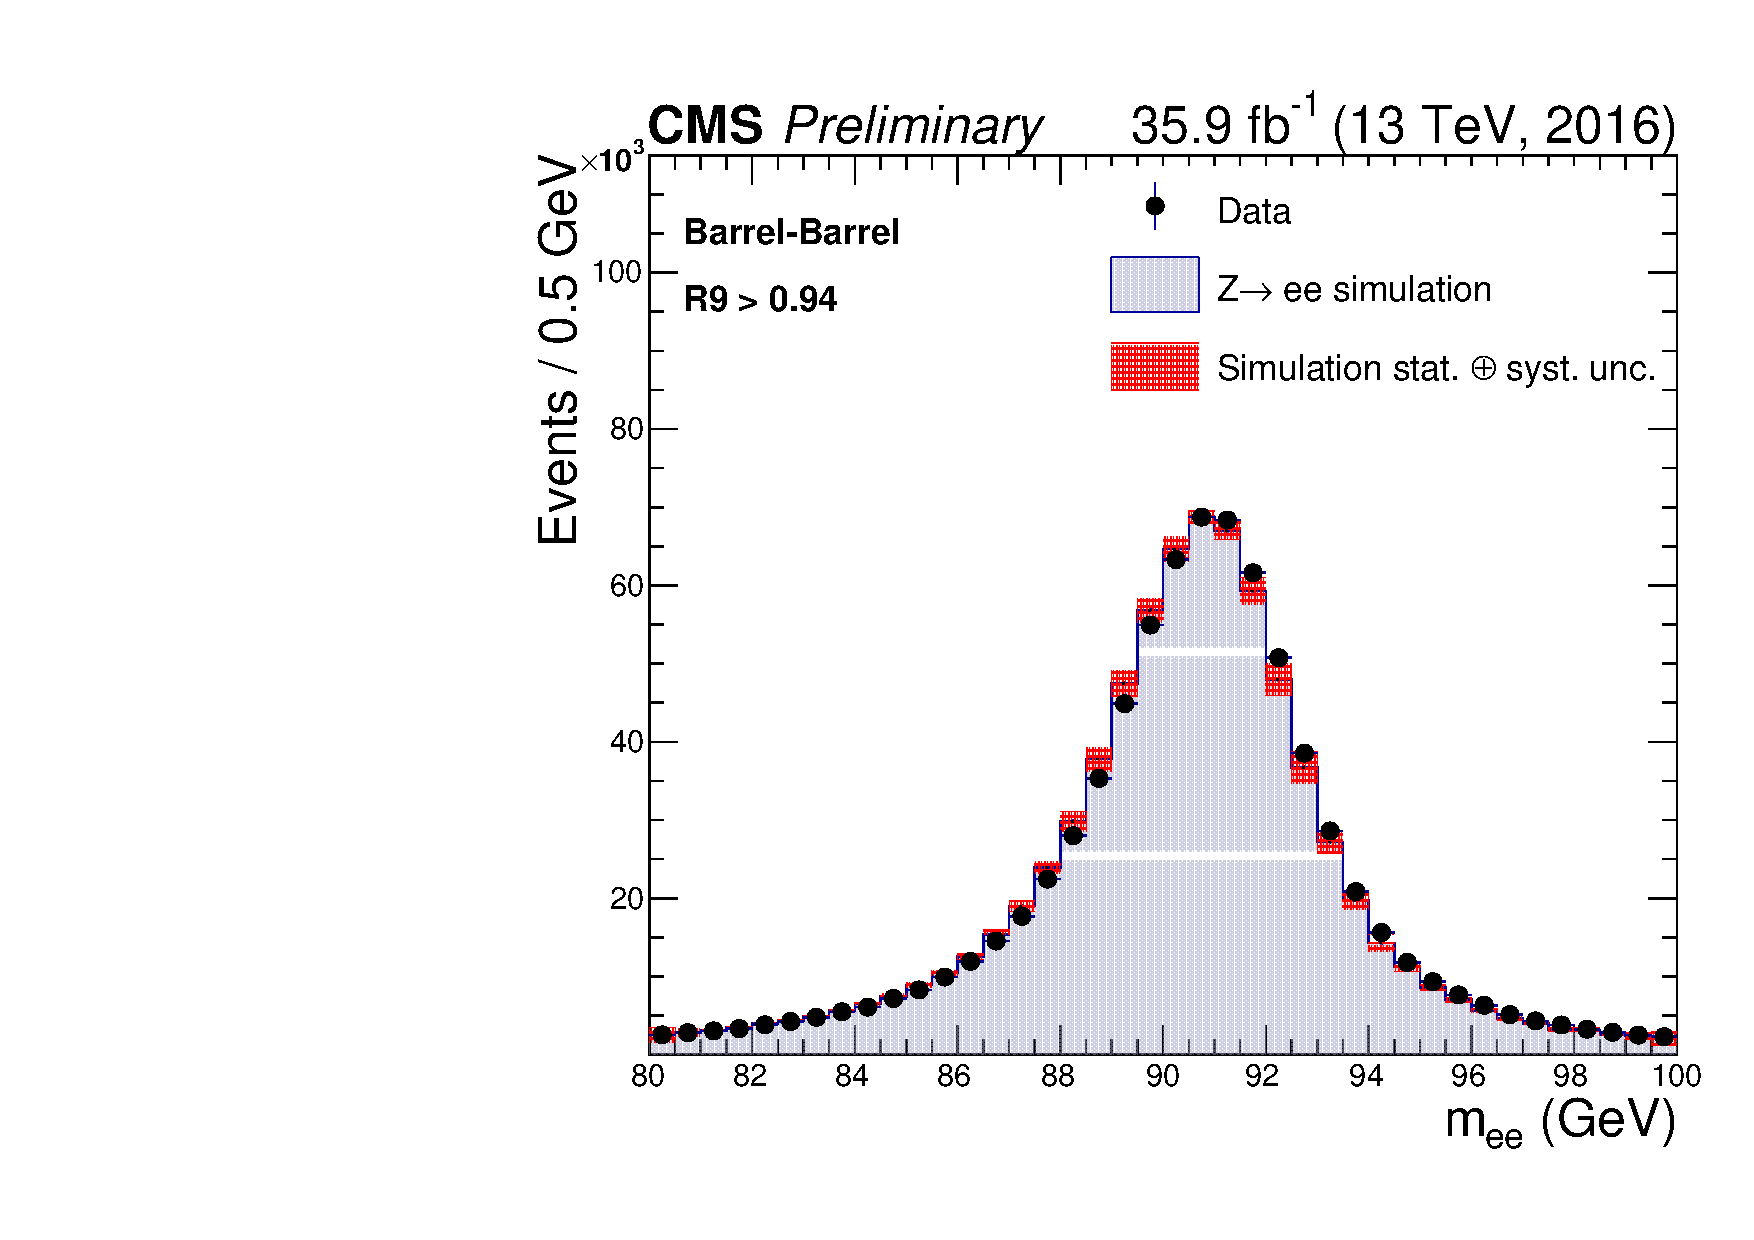
\includegraphics[width=0.49\textwidth]{Figures/Objects/meeBarrel2016}
  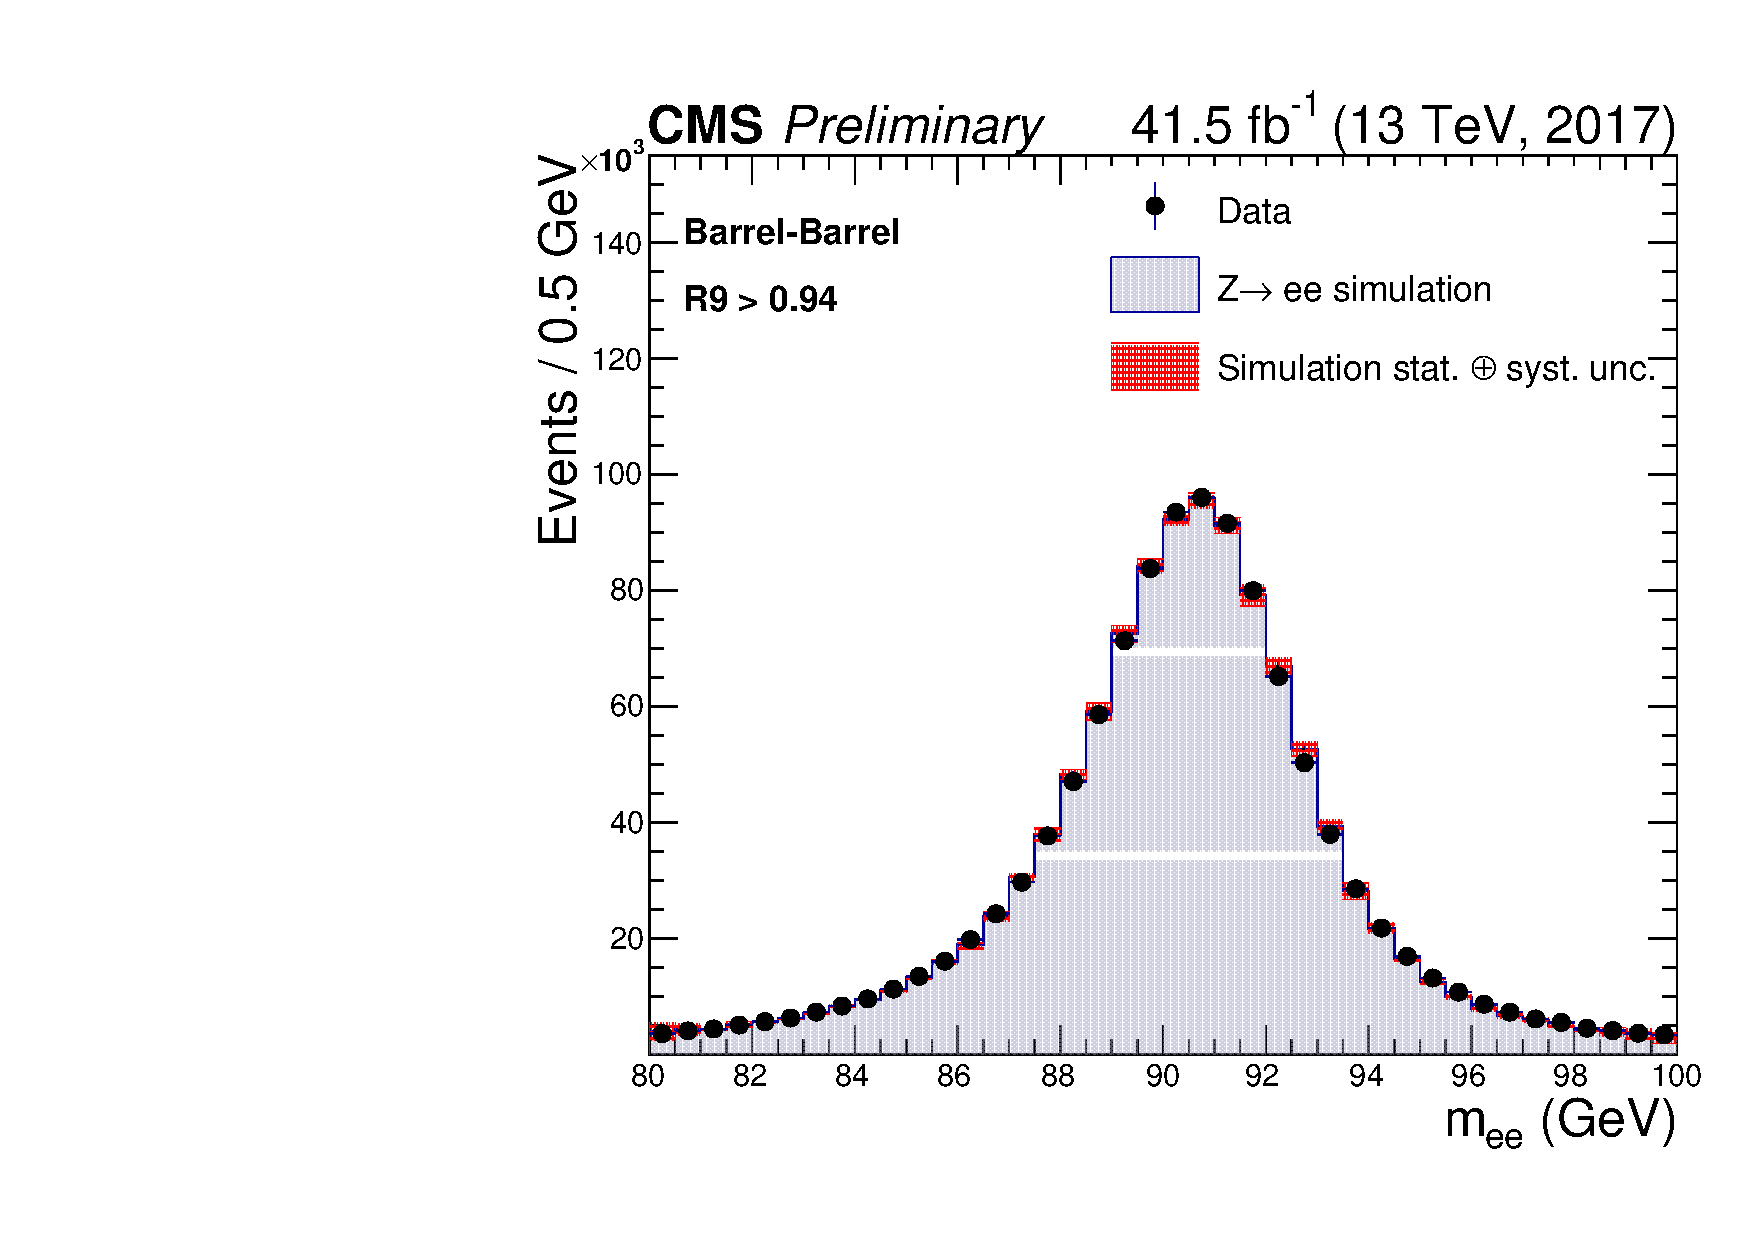
\includegraphics[width=0.49\textwidth]{Figures/Objects/meeBarrel2017} \\
  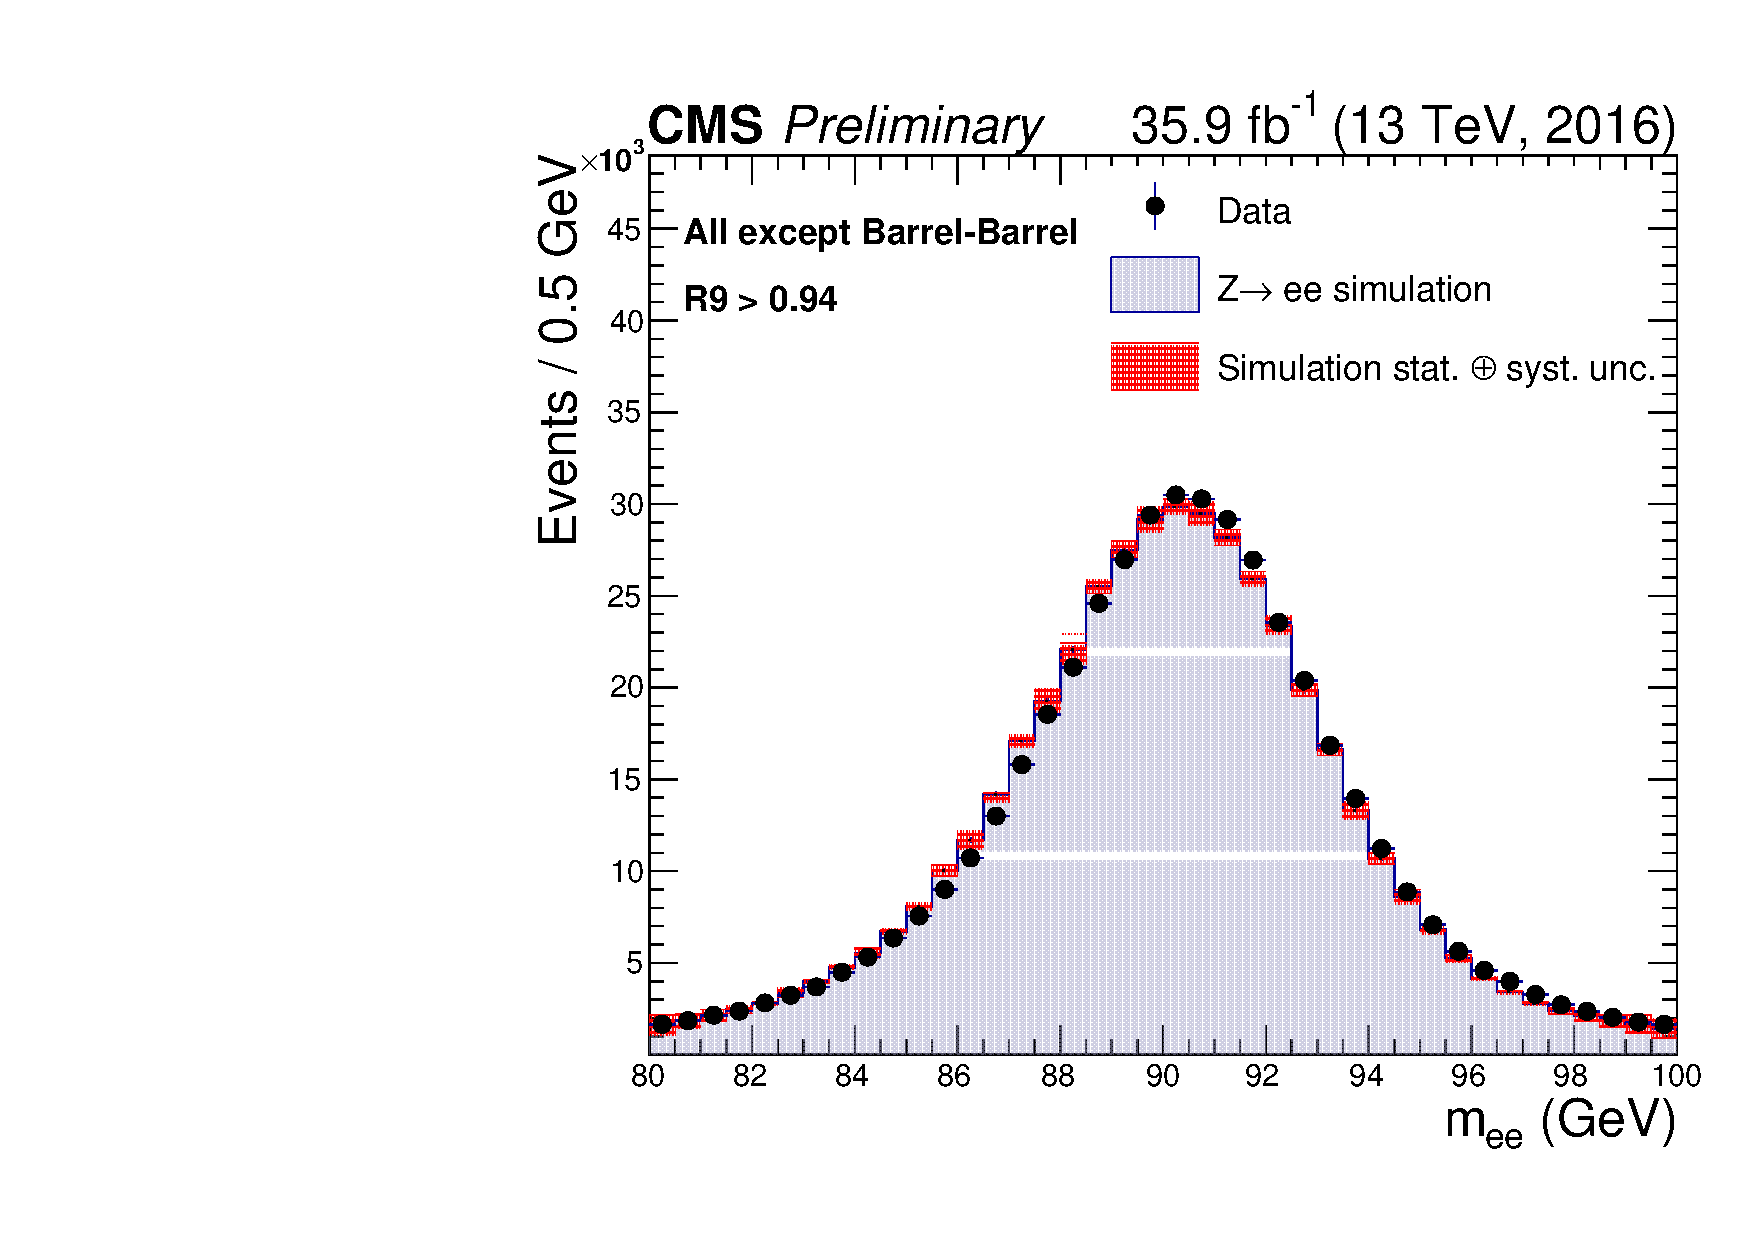
\includegraphics[width=0.49\textwidth]{Figures/Objects/meeEndcap2016}
  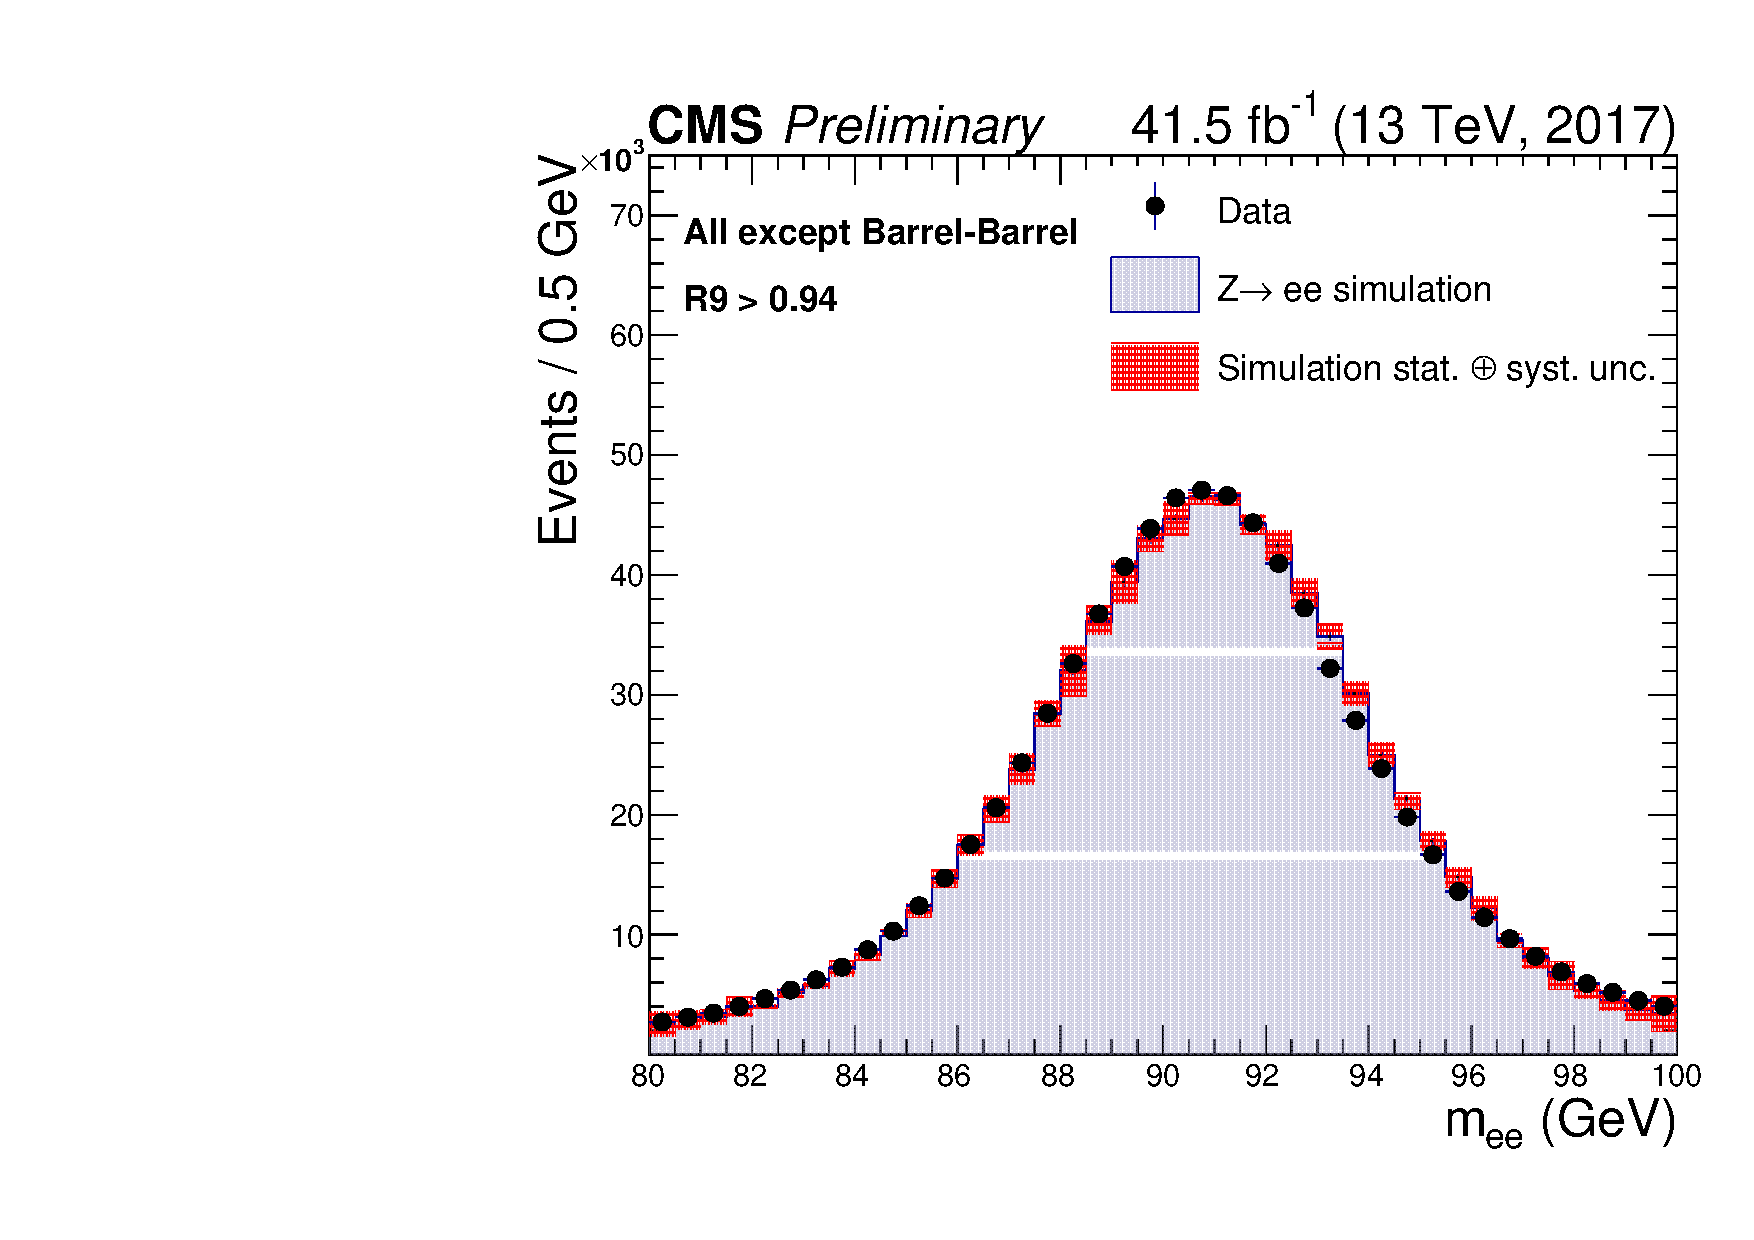
\includegraphics[width=0.49\textwidth]{Figures/Objects/meeEndcap2017}
  \caption[Dielectron invariant mass distributions.]
  {
    Comparison of the dielectron invariant mass distributions in data and simulation
    (after energy smearing) for \Zee
    events where electrons are reconstructed as photons.
    The \RNINE variable is required to be greater than 0.94.
    The simulated distributions are
    normalised to the integral of the data distribution 
    in the range $87 < m_{ee} < 93$ GeV to highlight
    the agreement in the bulk of the distributions.
    The comparison is shown for events where at both electrons are in the ECAL barrel (top), 
    and least one electron is not in the ECAL barrel (bottom).
    The plots on the left show data and simulation from 2016, 
    with 2017 data and simulation shown in the plots on the right~\cite{HIG-18-029}.
  }
  \label{fig:obj_mee}
\end{figure}

\subsection{Photon preselection}
\label{sec:objects_PhotonPresel}

To be further considered in the \Hgg analysis, 
photons must pass a set of criteria designed to reduce the contamination from objects faking photons.
This preselection is similar to, but more stringent than, that required at trigger level.
The full set of requirements is:
\begin{itemize}[noitemsep]
  \item to be within the ECAL acceptance; this means $|\eta|\,<\,2.5$ and excluding the endcap transition region $1.44\,<\,|\eta|\,<\,1.57$.
  \item passing the electron veto
  \item $\pt > 30 (20)$ GeV for the leading (subleading) photon in 2016. 
  The thresholds are 35 and 25 GeV respectively in 2017, due to the tighter trigger requirements.
  \item either $\mathcal{I}_{\text{ch}} < 20$ GeV, 
  or $\mathcal{I}_{\text{ch}} / \pt < 0.3$ for photons with $\RNINE < 0.8$.
  \item an additional set of \RNINE and $\eta$-dependant shower shape and isolation requirements, 
  summarised in Table~\ref{tab:obj_preselection}.
\end{itemize}

\begin{table}[htbp]
  \begin{center}
    \begin{tabular}{l|c|c|c|c|c}
      \hline
      \multicolumn{1}{c|}{} & \RNINE & H/E     & $\sigma_{\eta \eta}$ & $\mathcal{I}_{\text{ph}}$ & $\mathcal{I}_{\text{tk}}$ \\
      \hline
      \multirow{2}{*}{Barrel}
      & $[0.5, 0.85]$  & $<0.08$ & $<0.015$ & $<4.0$ & $<6.0$
      \\
      & $> 0.85$   & $<0.08$ & --       & -- & --
      \\ \hline
      \multirow{2}{*}{Endcaps}
      & $[0.8, 0.90]$  & $<0.08$ & $<0.035$ & $<4.0$ & $<6.0$
      \\
      & $> 0.90$     & $<0.08$ & --       & -- & --
      \\ \hline
    \end{tabular}
  \end{center}
  \caption[Summary of photon preselection requirements.]
  {
    Summary of photon preselection requirements.
  }
  \label{tab:obj_preselection}
\end{table}

The efficiency of these preselection criteria, aside from the electron veto, is measured using \Zee events.
To measure the electron veto efficiency, \Zmumug events are used.
Efficiencies range from over 94\% for high \RNINE photons in the barrel, 
to around 50\% for low \RNINE photons in the endcaps.
Very good agreement is observed between data and simulation. %0.1-0.3\% in barrel, 0.5-1\% in endcap

\subsection{Photon identification}
\label{sec:objects_PhotonIDBDT}

An additional part of the photon preselection is the photon identification BDT.
Its purpose is to discriminate between real photons and photon candidates passing the preselection which originate from other objects, 
such as jet fragments.
The BDT is trained using $\gamma$ + jet events passing the preselection described above, with real photons treated as signal and fake photons as background.
The inputs are similar to the those used in the energy regression, 
including shower shape and isolation variables.
In addition, pileup-sensitive variables $\rho$ and the number of interaction vertices, 
together with photon kinematic variables, are used as inputs.

A loose selection on the photon identification BDT at -0.9 completes the analysis preselection.
The output score on preselected diphoton events is shown in Figure~\ref{fig:obj_IDMVA}.
Additional validation using \Zee events is demonstrated in Figures~\ref{fig:obj_ZeeIDMVA}.

\begin{figure}[h!]
  \centering
  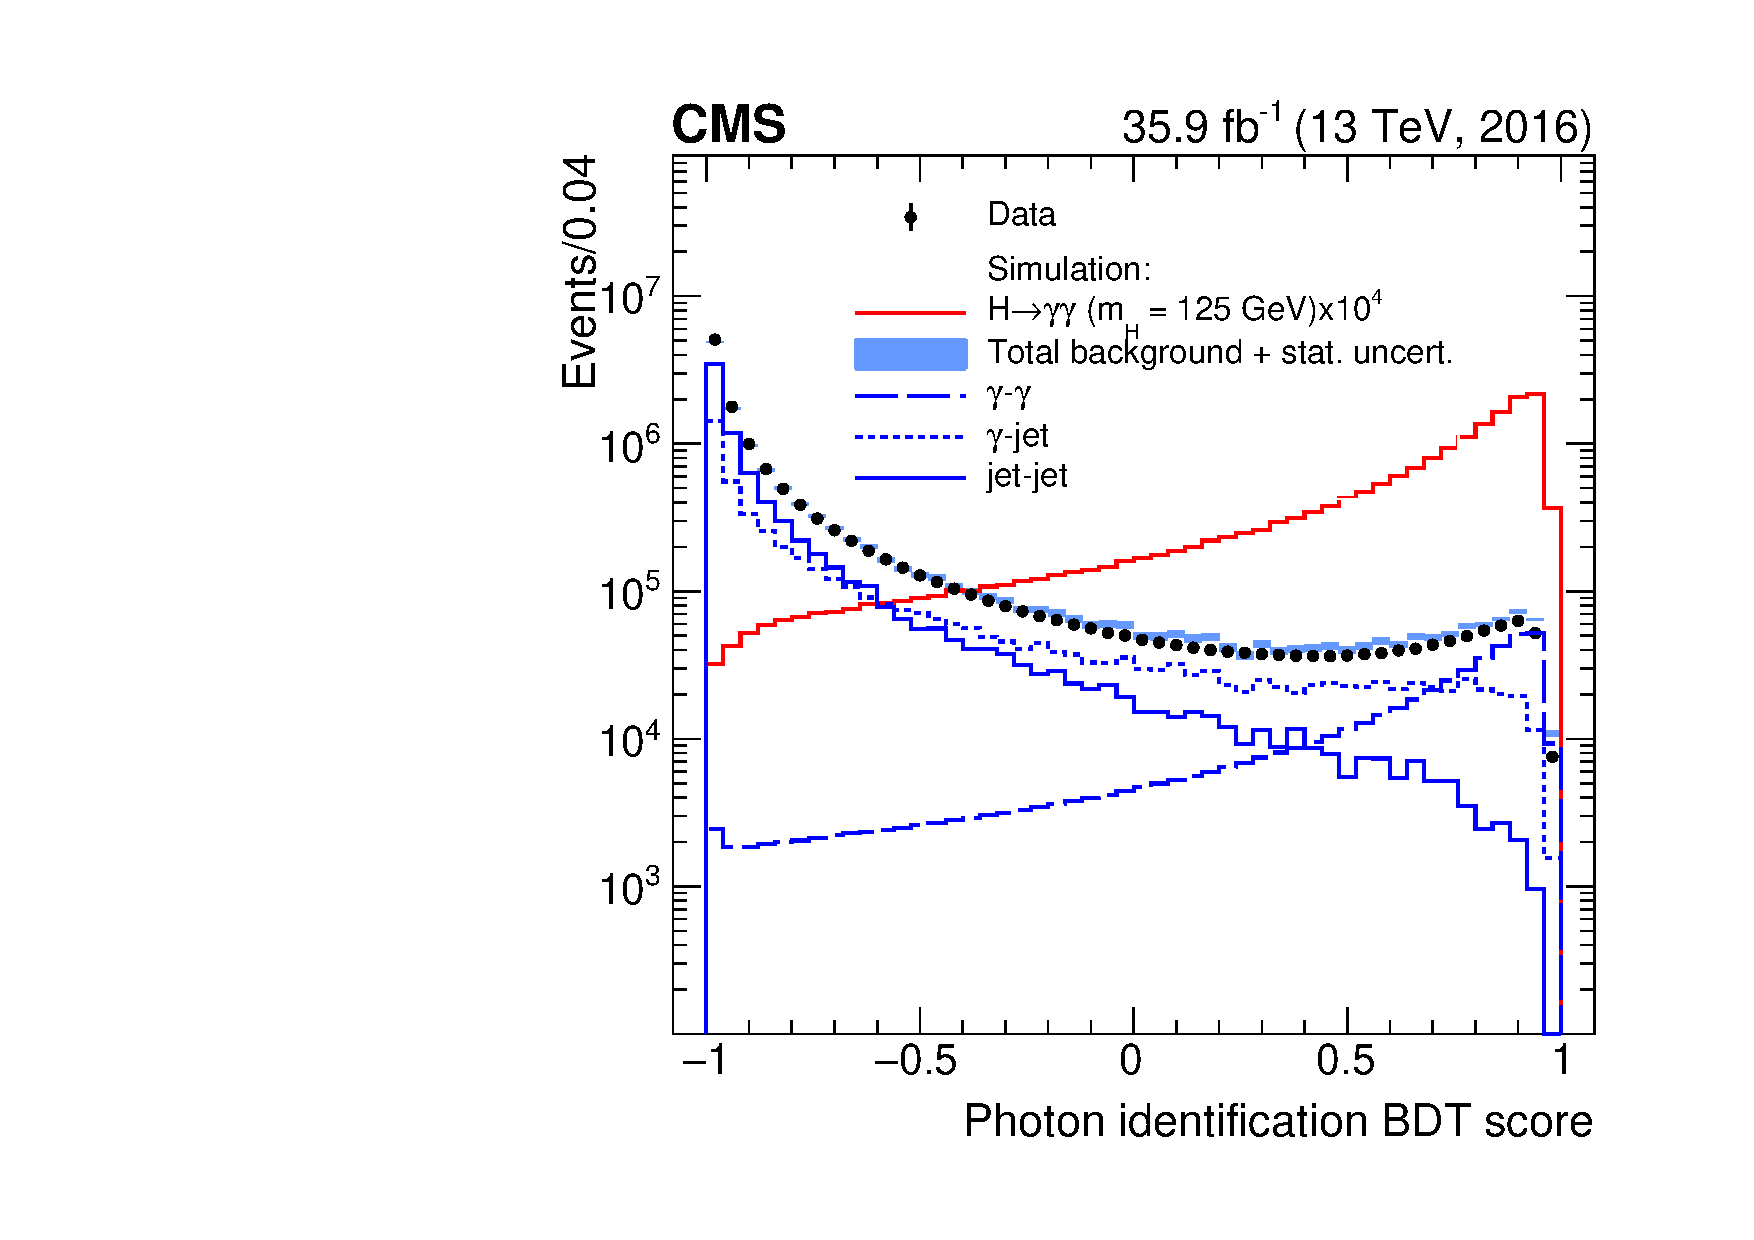
\includegraphics[width=0.49\textwidth]{Figures/Objects/IDMVA2016}
  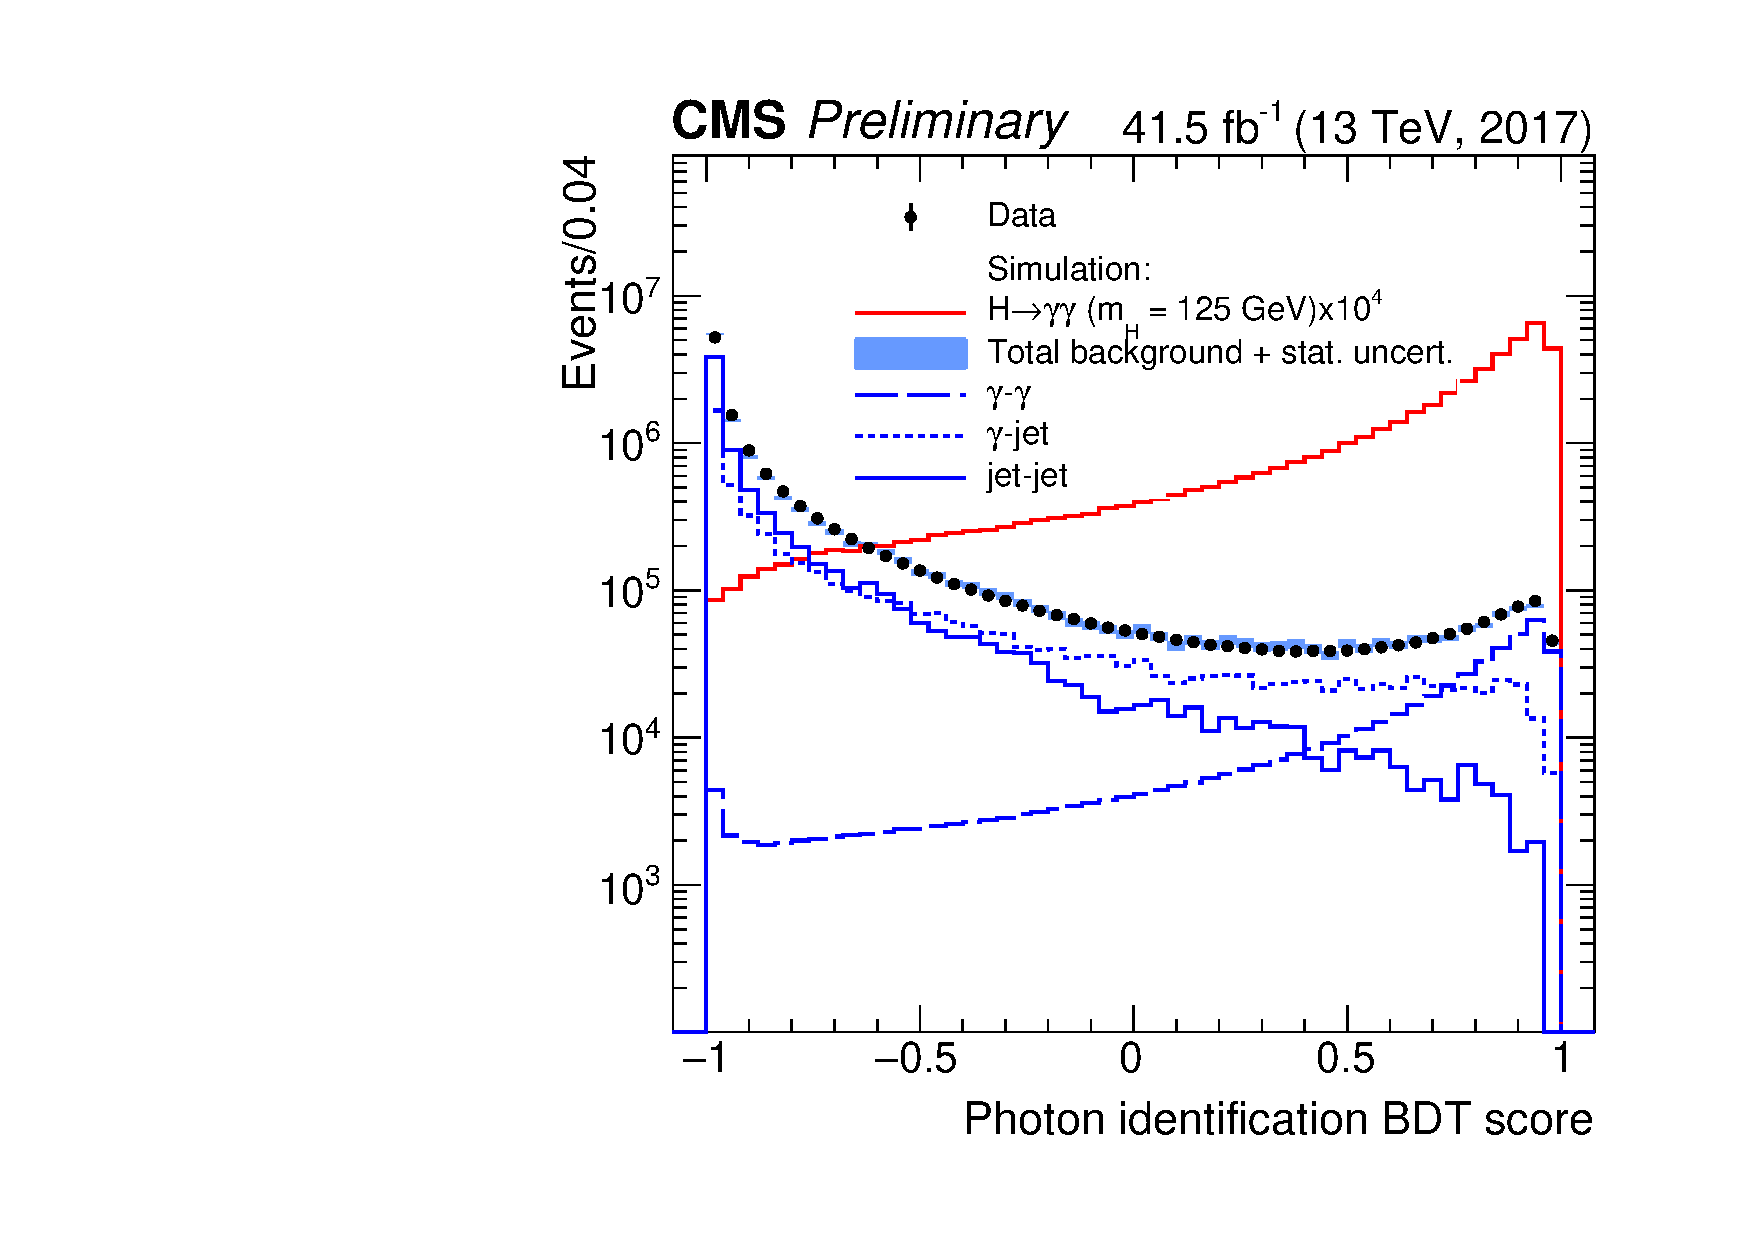
\includegraphics[width=0.49\textwidth]{Figures/Objects/IDMVA2017}
  \caption[Photon identification BDT score distributions.]
  {
    Distribution of the photon identification BDT score of the lowest scoring photon
    of diphoton pairs with an invariant mass in the range $100 < \mgg < \SI{180}{GeV}$, 
    for events passing the preselection in data (black points), 
    and for simulated background events (blue histogram). 
    Histograms are also shown for different components of the simulated background.
    The sum of all background distributions is scaled up to data. 
    The red histogram corresponds to simulated Higgs boson signal events. 
    The left figure shows 2016 data and simulation~\cite{HIG-16-040}, 
    with 2017 data and simulation shown on the right~\cite{HIG-18-029}.
  }
  \label{fig:obj_IDMVA}
\end{figure}

\begin{figure}[h!]
  \centering
  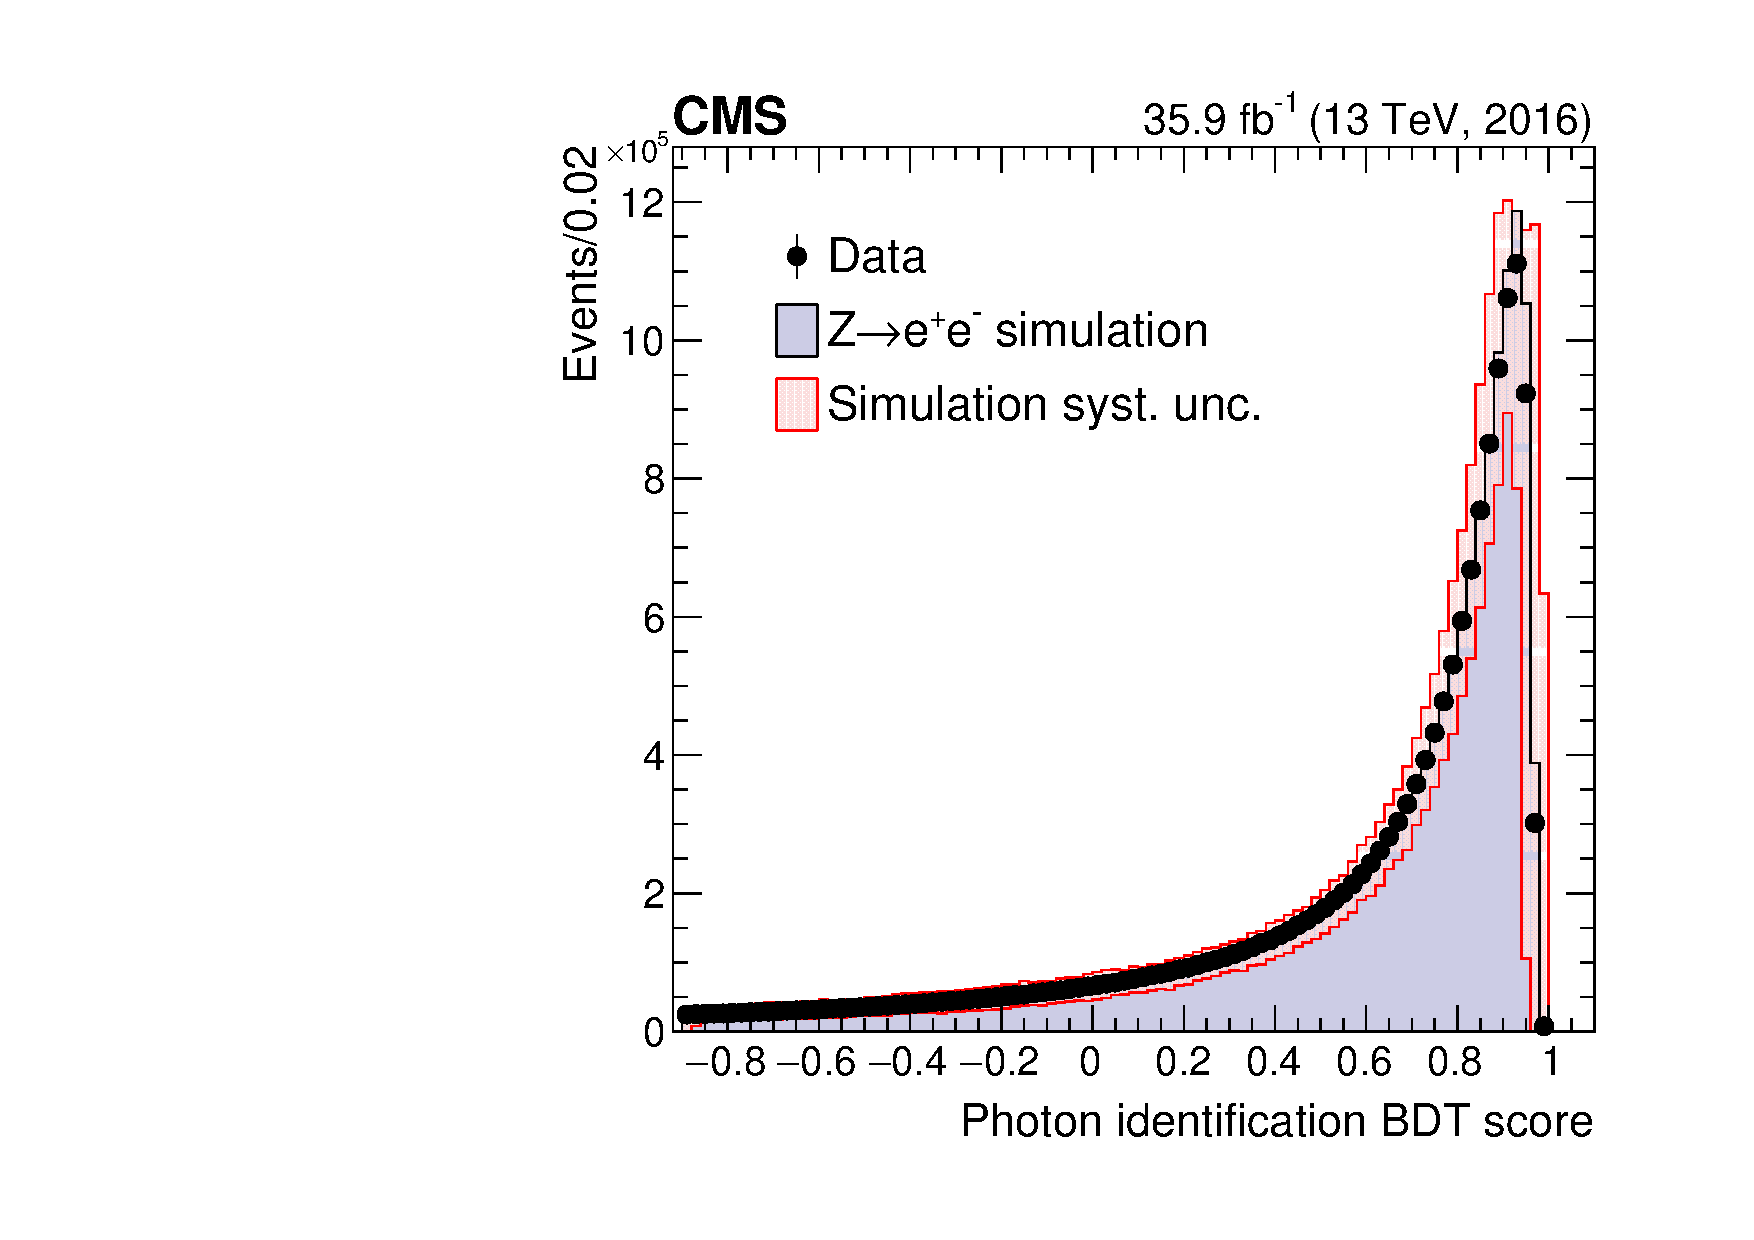
\includegraphics[width=0.49\textwidth]{Figures/Objects/ZeeIDMVA2016}
  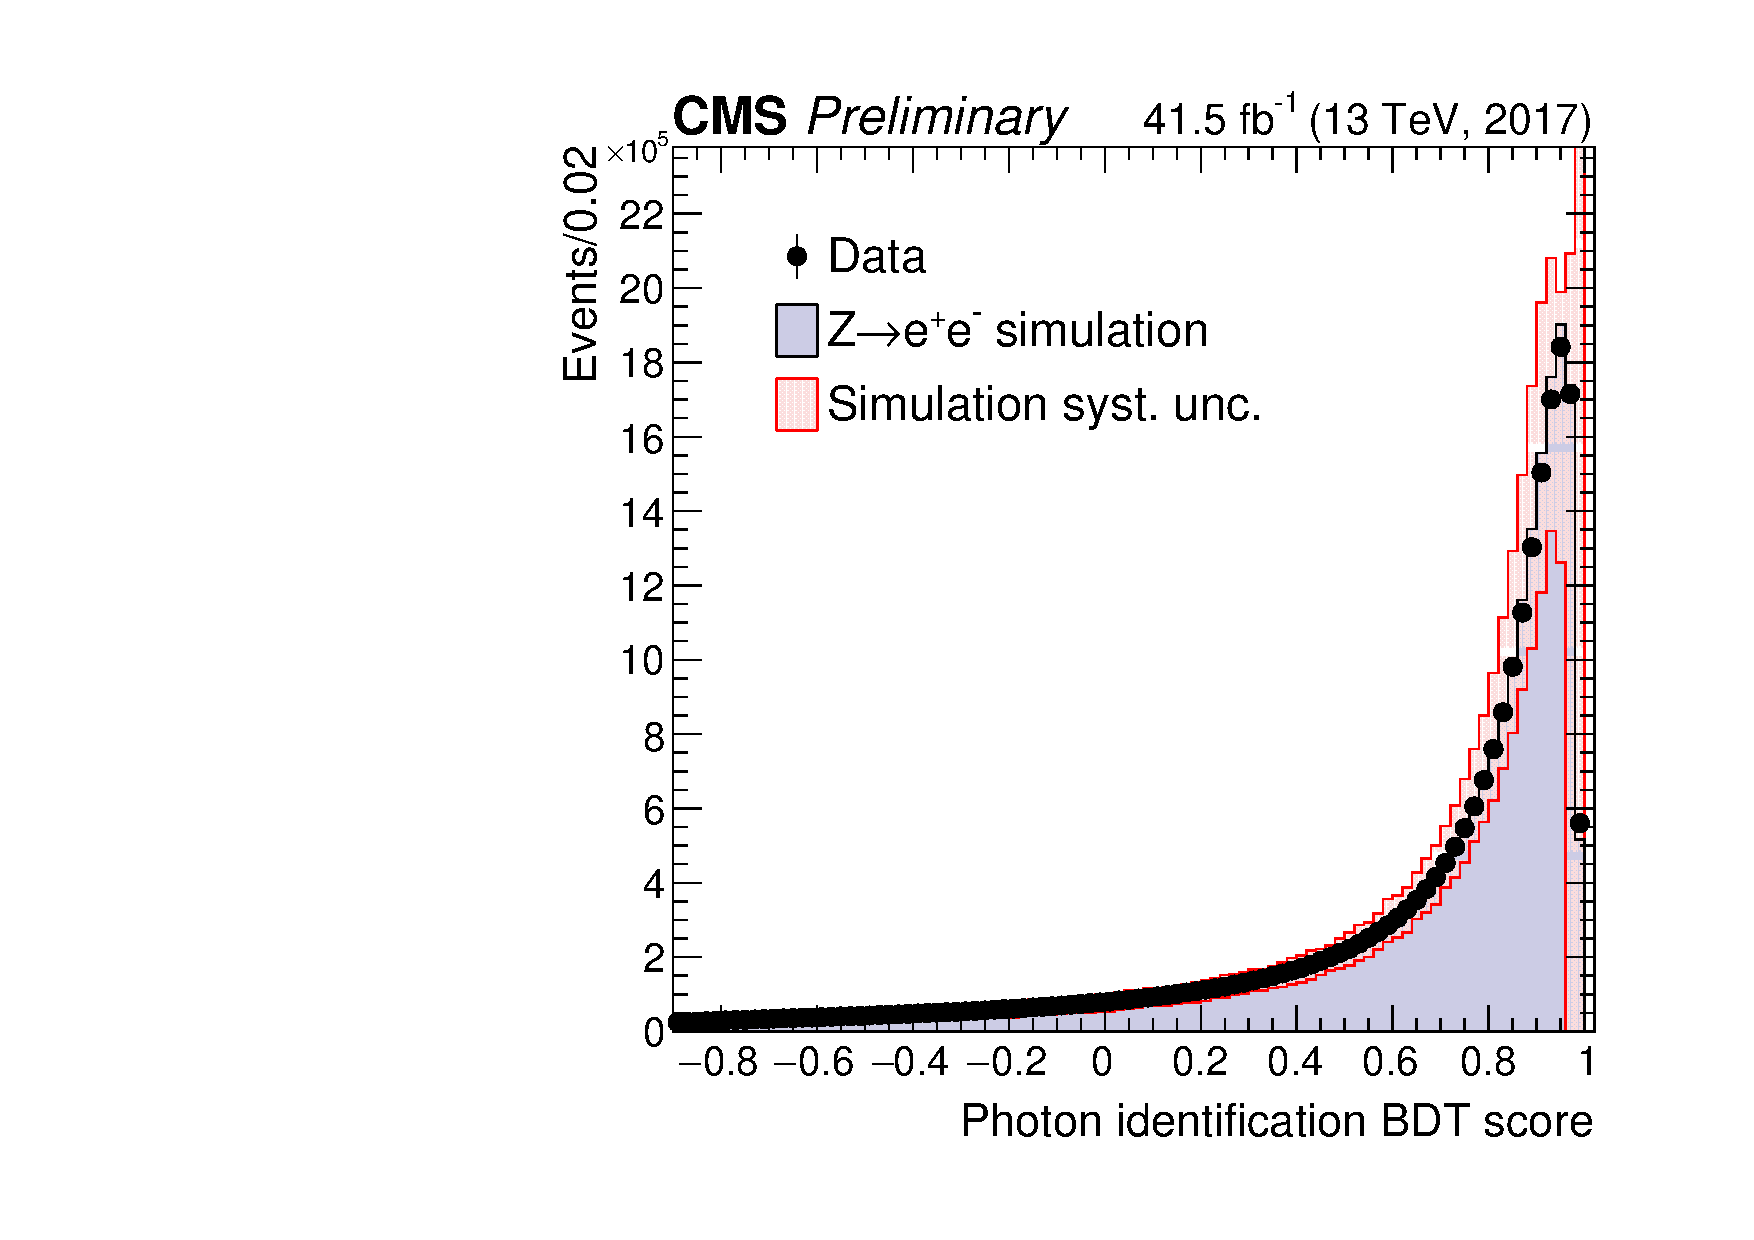
\includegraphics[width=0.49\textwidth]{Figures/Objects/ZeeIDMVA2017}
  \caption[Photon identification BDT score validation in \Zee events.]
  {
    Distribution of the photon identification BDT
    for \Zee events in data and simulation, where the electrons are reconstructed as photons. 
    The systematic uncertainty applied to the shape from simulation (hashed region) is also shown.
    The left figure shows 2016 data and simulation~\cite{HIG-16-040}, 
    with 2017 data and simulation shown on the right~\cite{HIG-18-029}.
  }
  \label{fig:obj_ZeeIDMVA}
\end{figure}

\section{Vertex reconstruction}

As can be seen in Equation~\ref{eq:obj_mgg}, 
the only parameters affecting the diphoton mass are the photon energies and the opening angle between them.
Since there are multiple p-p interactions at each bunch crossing, multiple vertices are present in each event, spread along the $z$-axis.
The choice of the vertex from which the diphoton originated has a direct impact on the angle $\theta$, 
and therefore the diphoton mass resolution.
Provided the chosen vertex is within ~\SI{1}{cm} of the true interaction vertex,
the mass resolution is dominated by the photon energy resolution and the contribution from the angle is negligible.
A BDT is therefore trained to identify the most likely diphoton interaction vertex.

\subsection{Vertex selection}

The vertex identification BDT is trained with simulated \Hgg signal events, 
with the objective of selecting the true interaction vertex.
Since photons do not produce tracks, its inputs are variables related to tracks
recoiling against the diphoton system.
The variables are calculated for each candidate vertex, and are defined as follows:
\begin{itemize}
        \item $\sum_{i}|\vec{p}_T^{i}|^{2}$,
        \item $\displaystyle -\sum_{i}(\vec{p}_T^{i}\cdot \frac{\vec{p}_T^{\gamma\gamma}}{|\vec{p}_T^{\gamma\gamma}|})$,
        \item $(|\sum_{i}\vec{p}_T^{i}| - \pt^{\gamma\gamma})/(|\sum_{i}\vec{p}_T^{i}| + \pt^{\gamma\gamma})$,
\end{itemize}
where $\vec{p}_T^{i}$ is the \pt of the $i$-th track
associated with a given vertex 
and $\vec{p}_T^{\gamma\gamma}$ is the vector representing the diphoton transverse momentum.

If one or more of the photons have converted into electrons in the tracker, 
two more variables are used in addition to those above:
\begin{itemize}
        \item the number of conversions,
        \item the pull $|z_{\text{vtx}} - z_e| /\sigma_{z}$ between the
                longitudinal position of the reconstructed vertex,
                $z_{\text{vtx}}$, and the longitudinal position of the
                vertex estimated using conversion track(s), $z_e$,
                where the variable $\sigma_{z}$ denotes the uncertainty 
                on $z_e$.
\end{itemize}

The vertex with the highest vertex identification BDT output score is then chosen 
as the \Hgg interaction point.
This choice is considered to be the ``correct" vertex if the distance from the true interaction vertex
is less than \SI{1}{cm}, and is used to define the vertex choice efficiency.
The inclusive efficiency is approximately 82\% in 2016 conditions, %TODO define inclusive?
decreasing only slightly to 81\% in 2017 conditions.
This shows that the vertex identification procedure is robust to increases in pileup.
It also represents a substantial improvement compared to the default CMS vertex, %chosen using largest sum of squared track pT
which is correct in around 74\% of events.
%WV worsens resolution by about 1 GeV

The performance of the vertex identification BDT is
validated using $\Zmumu$ events.
The tracks from the muons are ignored in order to mimic the diphoton system.
Comparison between data and simulation in these events is shown in Figure~\ref{fig:obj_VtxId}.

\begin{figure}[h!]
  \centering
  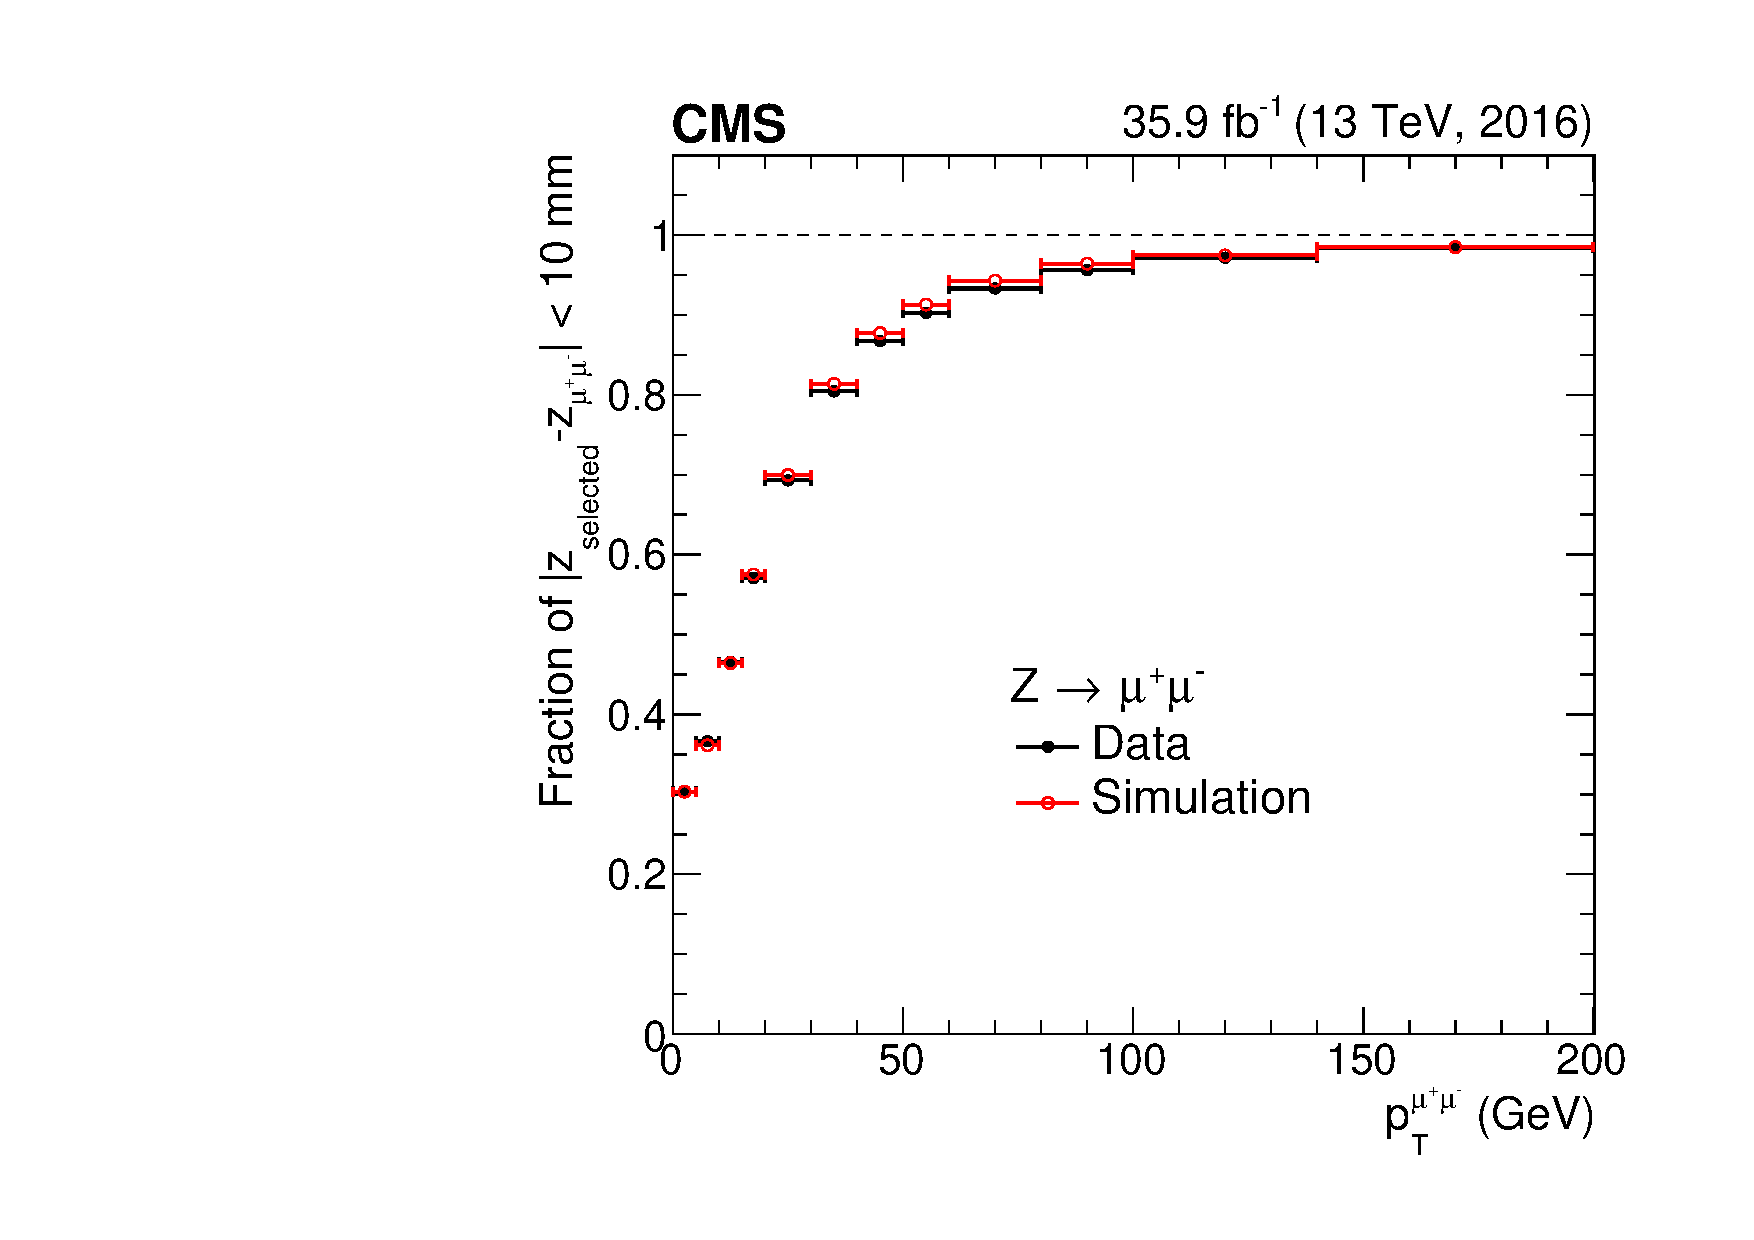
\includegraphics[width=0.49\textwidth]{Figures/Objects/VtxId2016}
  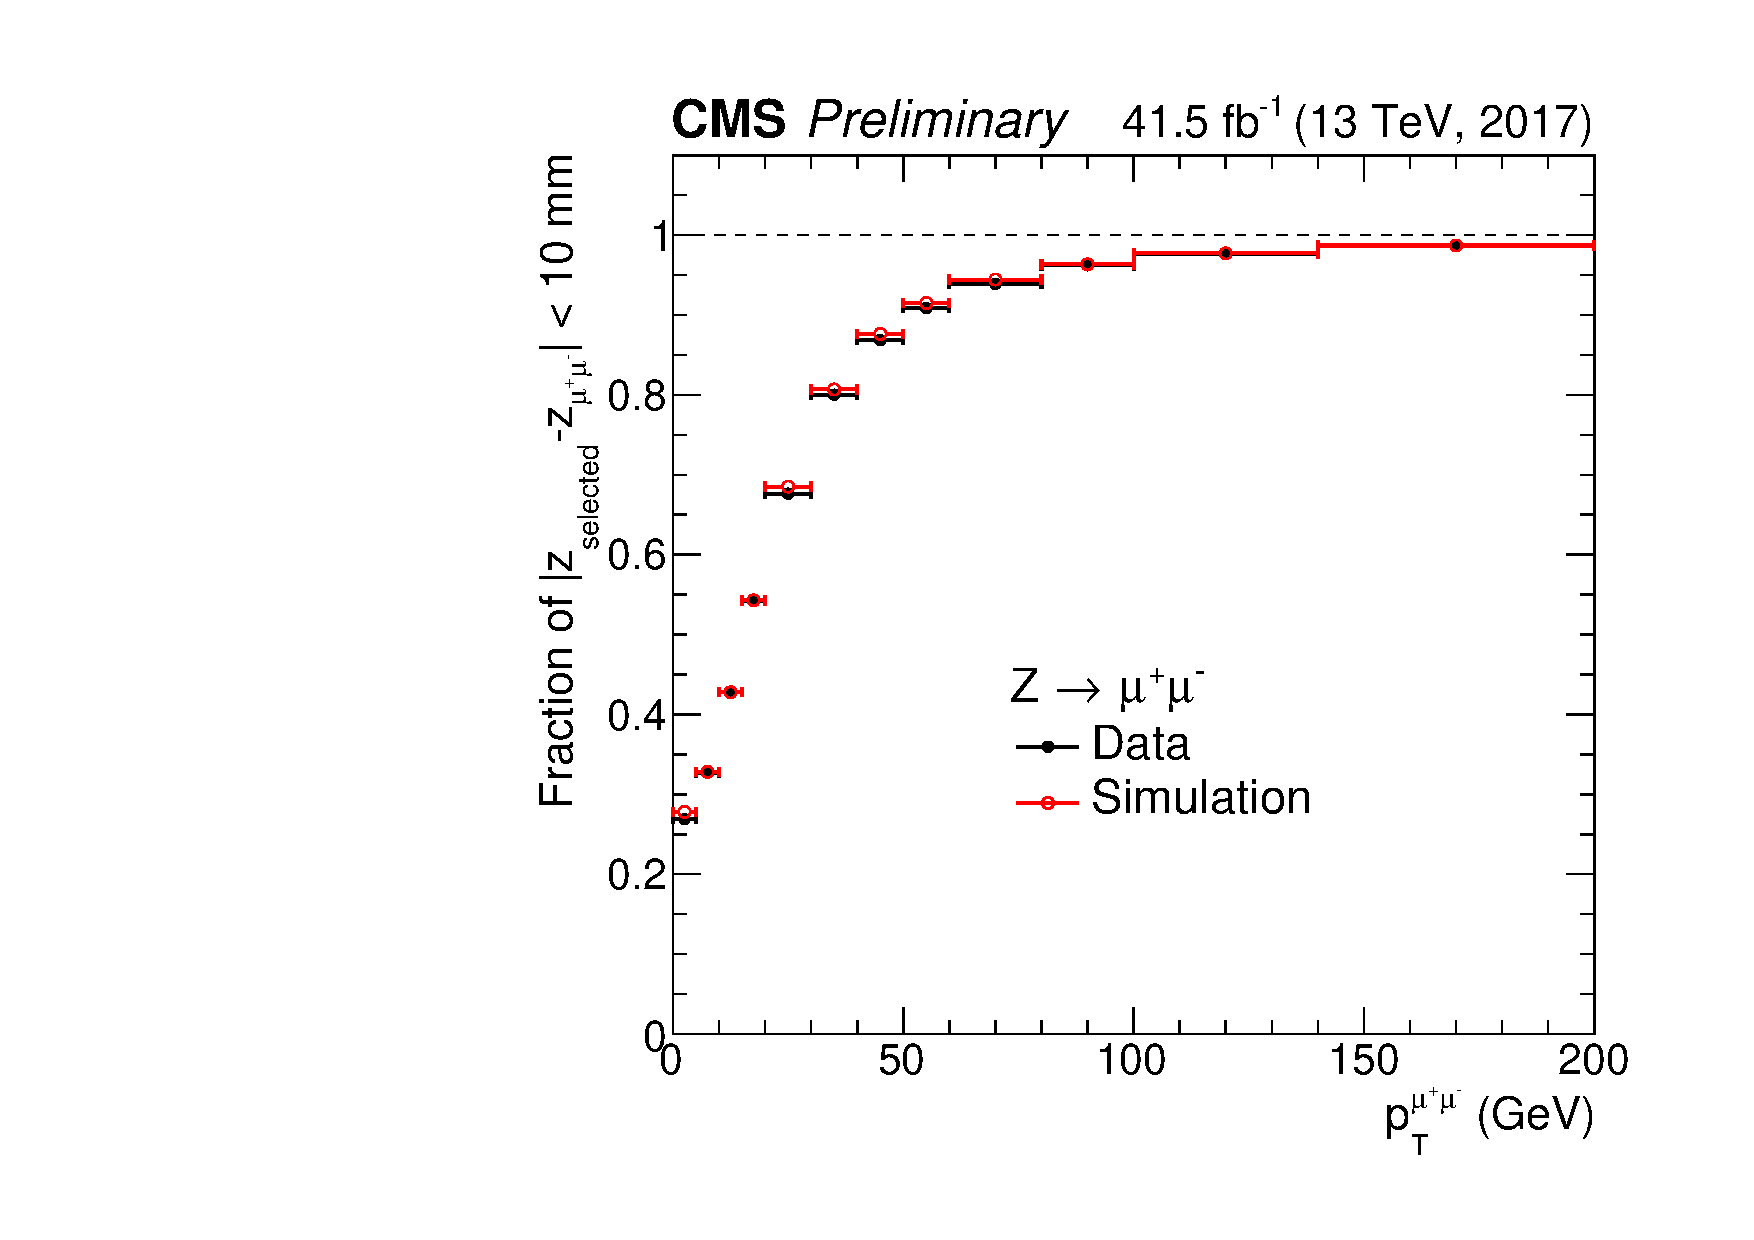
\includegraphics[width=0.49\textwidth]{Figures/Objects/VtxId2017}
  \caption[Vertex identification validation in \Zmumu events.]
  {
    Validation of the \Hgg vertex identification algorithm on \Zmumu events
    omitting the muon tracks. 
    Simulated events are weighted to match the distributions of pileup
    and location of primary vertices in data.
    The left figure shows 2016 data and simulation~\cite{HIG-16-040}, 
    with 2017 data and simulation shown on the right~\cite{HIG-18-029}.
  }
  \label{fig:obj_VtxId}
\end{figure}

\subsection{Vertex probability}

A second vertex-related multivariate discriminant (vertex probability BDT),
is designed to estimate, event-by-event, the probability for the vertex
assignment to be within \SI{1}{cm} of the diphoton interaction point
and thus considered ``correct".
The vertex probability BDT is trained on simulated $\Hgg$ events using
the following input variables:
\begin{itemize}
        \item the number of vertices in each event,
        \item the values of the vertex identification BDT score for
                the three most probable vertices in each event,
        \item the distances between the chosen vertex and the second and
                third choices,
        \item the transverse momentum of the diphoton system, $\pt^{\gamma\gamma}$,
        \item the number of photons with an associated conversion track.
\end{itemize}

\begin{figure}[h!]
  \centering
  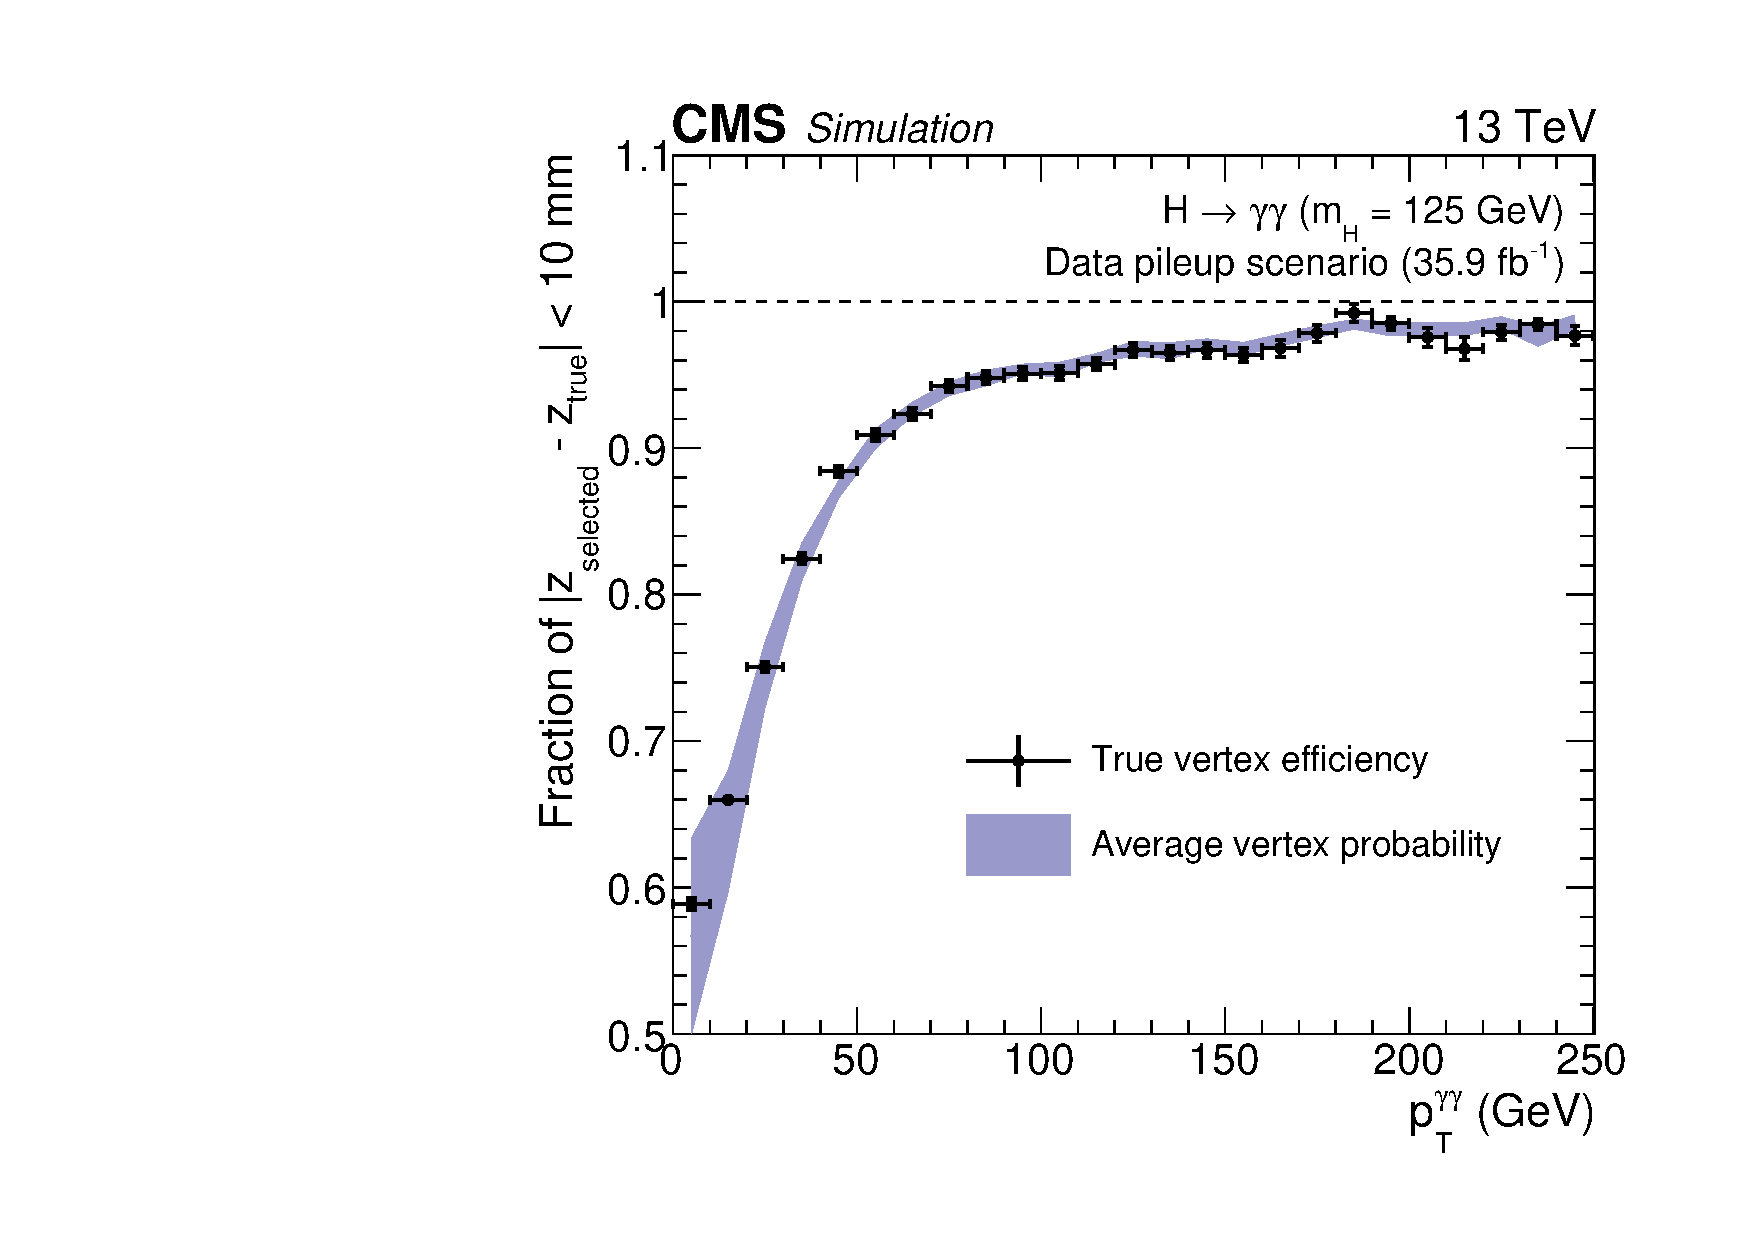
\includegraphics[width=0.49\textwidth]{Figures/Objects/VtxProbPt2016}
  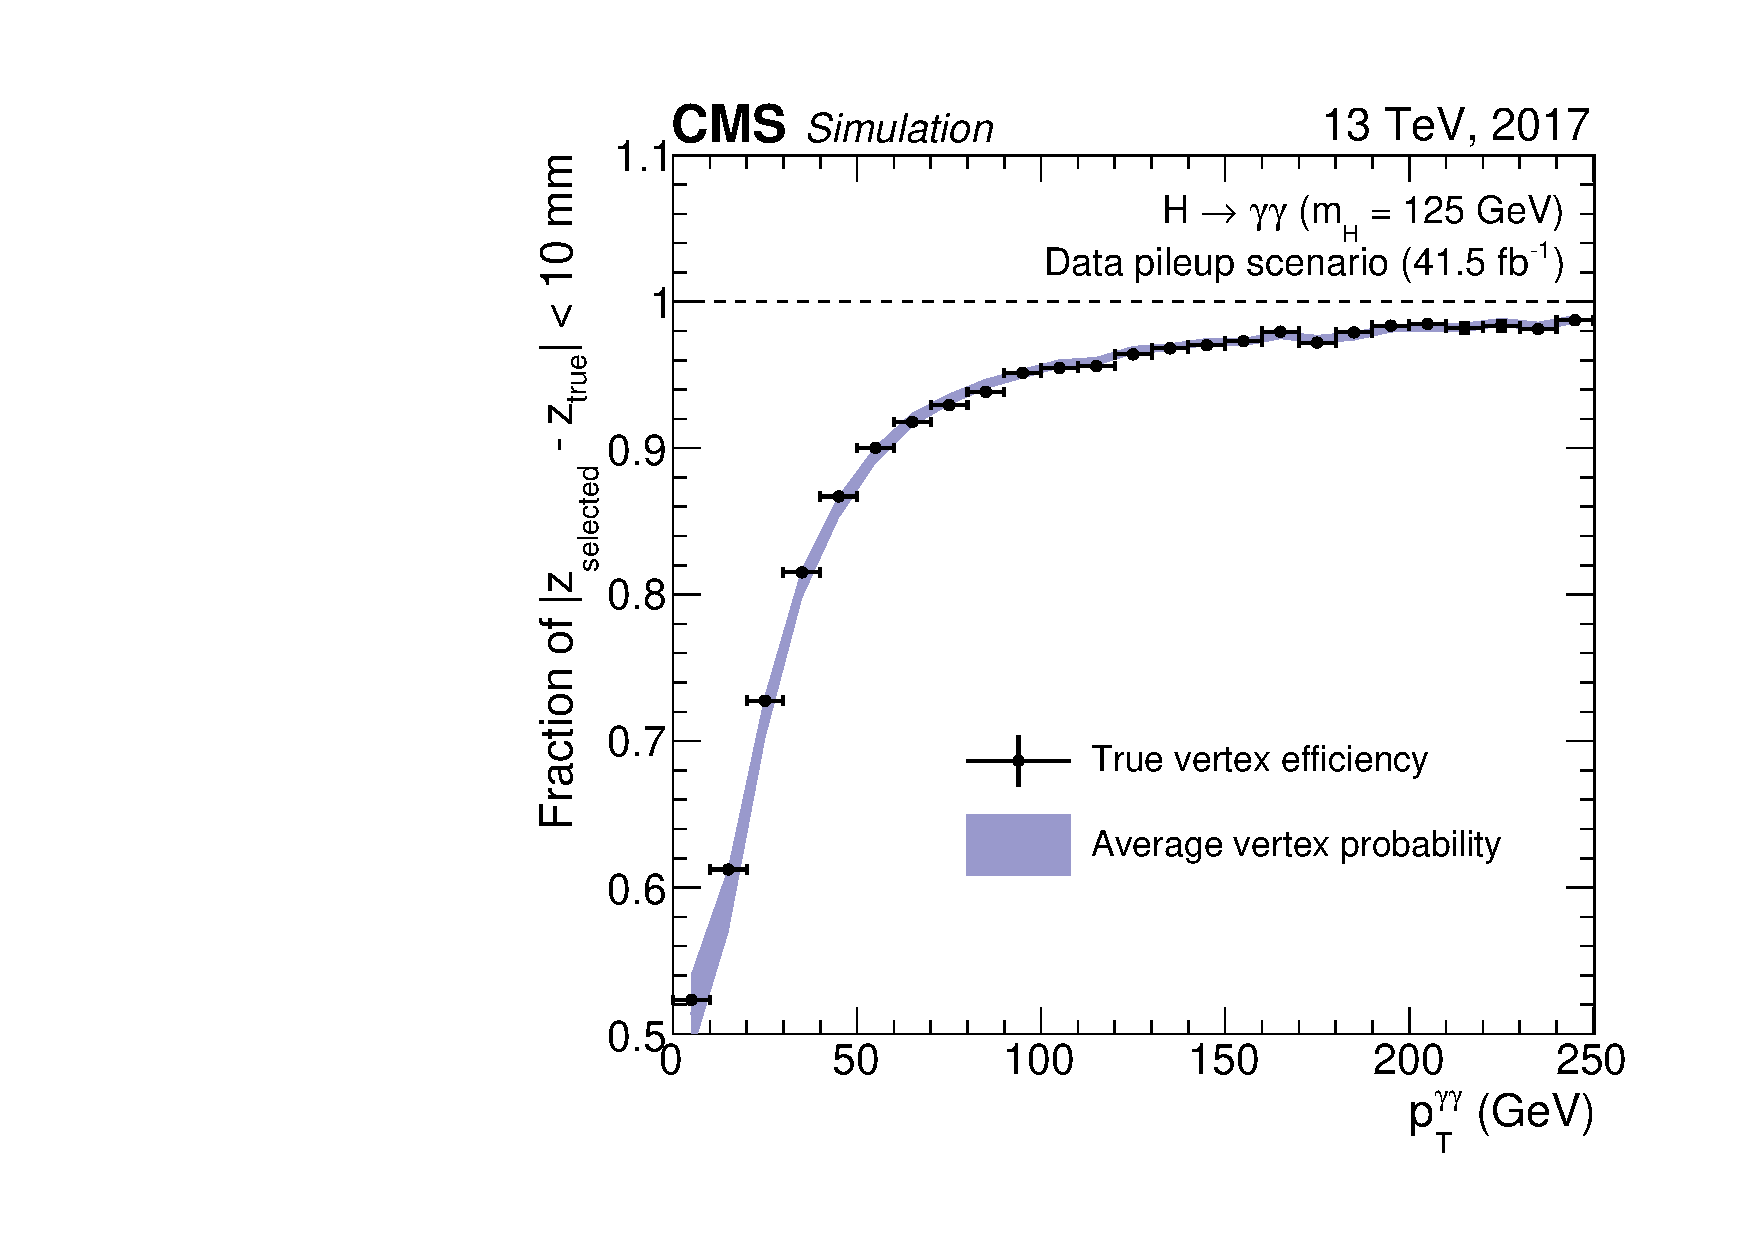
\includegraphics[width=0.49\textwidth]{Figures/Objects/VtxProbPt2017} \\
  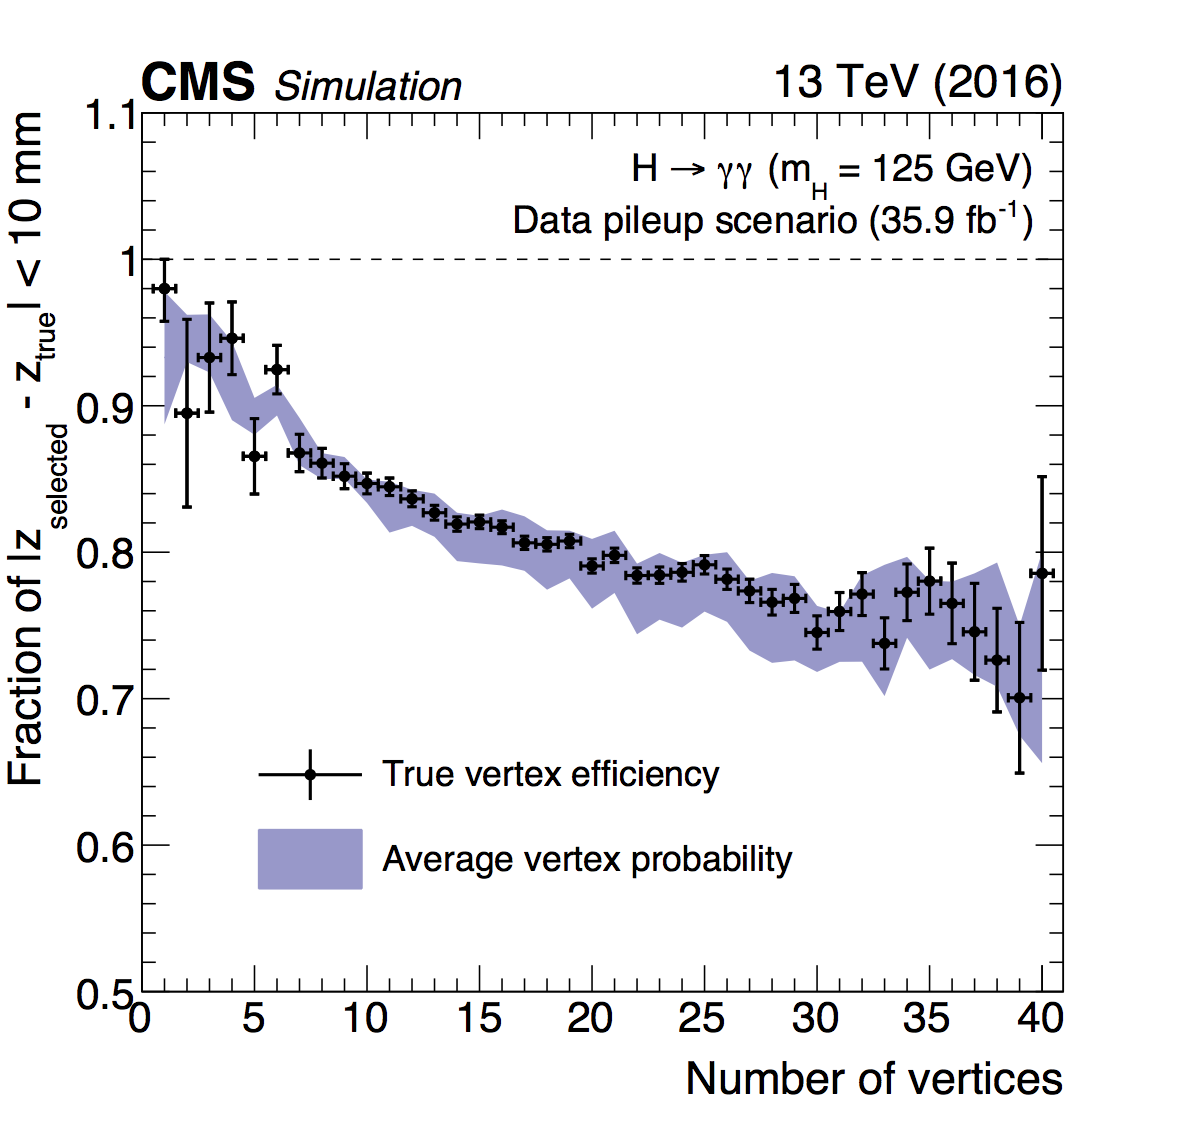
\includegraphics[width=0.49\textwidth]{Figures/Objects/VtxProbNvtx2016}
  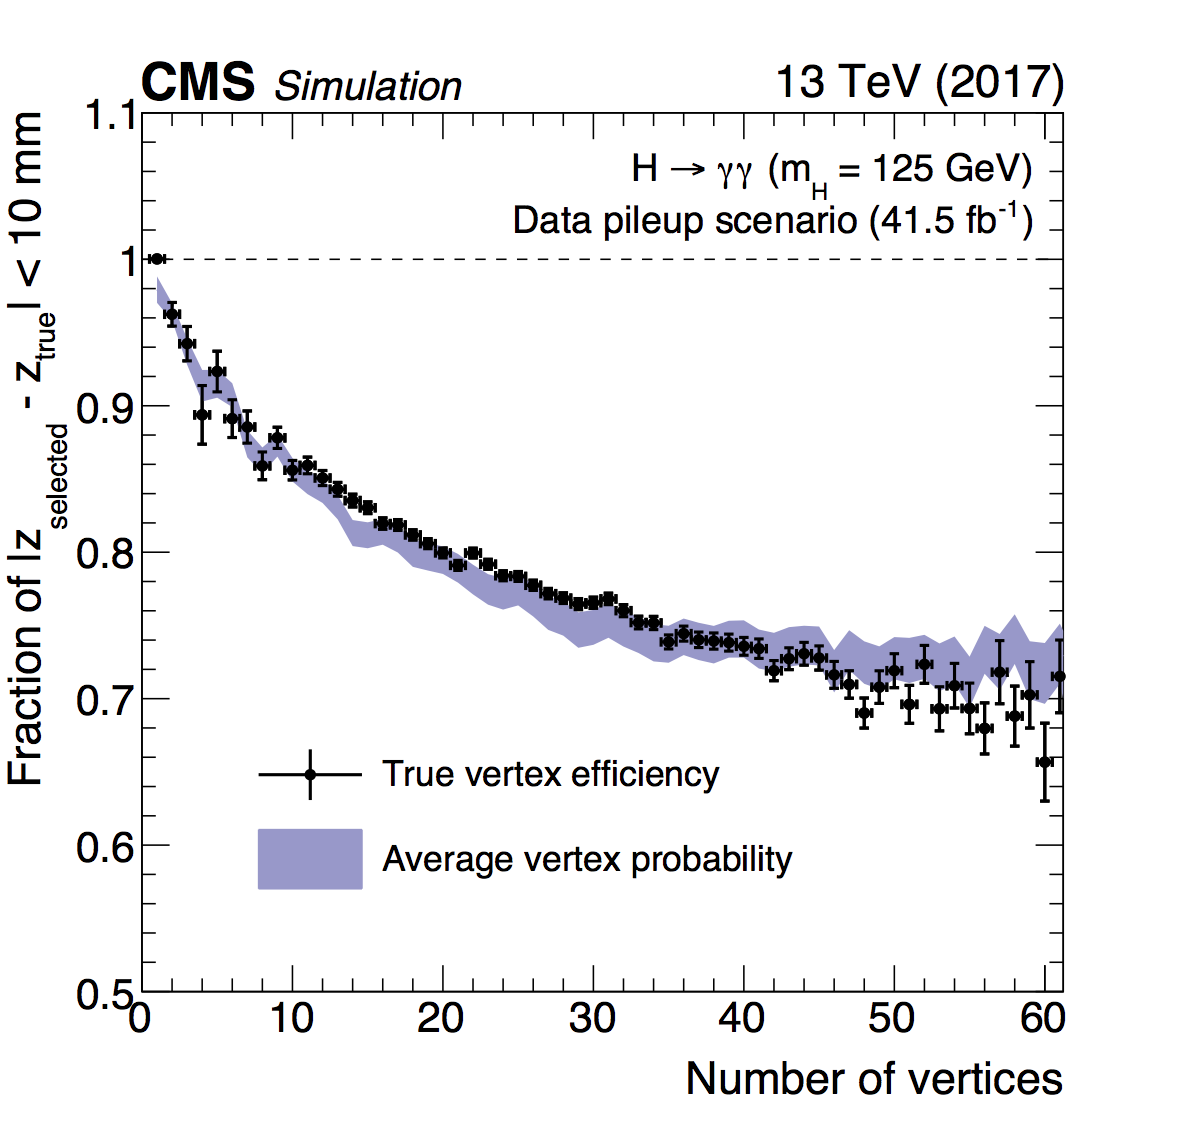
\includegraphics[width=0.49\textwidth]{Figures/Objects/VtxProbNvtx2017}
  \caption[Vertex probability validation in simulated \Hgg events.]
  {
    Comparison of the true vertex identification efficiency and the average estimated
    vertex probability as a function of the reconstructed diphoton \pt (top) and of the number of
    primary vertices (bottom) in simulated \Hgg events with $\mH = \SI{125}{GeV}$. Events are weighted
    according to the cross sections of the different production modes and to match the distributions
    of pileup and location of primary vertices in data.
    The plots on the left show simulation under 2016 conditions~\cite{HIG-16-040}, 
    with simulation under 2017 conditions shown in the plots on the right~\cite{HIG-18-029}.
  }
  \label{fig:obj_VtxProb}
\end{figure}

The vertex choice efficiency, together with the estimated vertex probability,
in simulated \Hgg signal events is shown in Figure~\ref{fig:obj_VtxProb}.
The simulated performance is shown as a function of both the \pt of the diphoton
system and of the number of vertices in the event.

\section{Jet reconstruction}

The collimated collection of particles produced by the hadronisation of quarks or gluons are referred to as jets.
Around 60\% of the average jet energy comes from charged hadrons, whose energy is well-measured by the tracker,
and another 30\% from photons, whose energy is measured precisely by the ECAL.
The remaining 10\% of energy from neutral hadrons is measured with worse resolution by the HCAL.
Jets are important in the \Hgg analysis because they enter the definition of the STXS signal bin definitions, 
are used to categorise the events targeting those bins, 
and are used to differentiate between production modes.

At CMS jets are formed using the \akt clustering algorithm~\cite{AntiKt} with distance parameter $R=0.4$. % check definitions of infrared and collinear safe etc
It is an iterative algorithm that defines a distance metric dependent on the \pt and angular parameters of candidate clusters of energy deposits, 
and groups together these clusters starting with the nearest two objects.
Once the shortest distance is between an object and the beampipe, the process stops and the clustered objects defined as a jet.
This is then repeated until all clusters have been collected into jets.

The inputs to the \akt algorithm are PF candidates with charged hadron subtraction (CHS)~\cite{JEC}. 
CHS reduces the contribution from pileup by identifying any charged hadrons associated with vertices other than the primary vertex.
Since the tracker coverage extends only to $|\eta|=2.5$, 
jets further forward than this do not have pileup removed via CHS.
Once the jets have been constructed, a set of corrections are applied to correct the jet energy scale and resolution in both data and simulation.
The correction procedure can be summarised as~\cite{JEC}:
\begin{itemize}
  \item corrections are made for the pileup contribution to jets, as a function of the event energy density, 
        and the jet \pt, $\eta$ and area.
        Any remaining differences between data and MC are derived after these corrections using pileup-only events.
  \item the reconstructed jet energy is corrected to agree with the true jet energy in both data and MC.
        This is performed as a function of \pt and $\eta$ to account for variation in response across the detector.
  \item residual differences between data and MC are corrected in two steps.
        First $\eta$-dependent corrections are applied using dijet events, 
        where the scale of a jet is corrected using a jet of similar \pt in the reference, well-measured $\eta < 1.3$ region.
        The \pt-dependent corrections are derived using events with a jet recoiling against a photon or $Z$ boson.
        This corrects the absolute scale of the jet.
  %\item finally, corrections dependent on the jet flavour are applied.%state optional? if not look up
\end{itemize}
%The final uncertainties on the jet energy scale are below 3% across the phase space considered
%by most analyses (pT > 30 GeV and |η| < 5.0). In the barrel region we reach an uncertainty
%below 1% for pT > 30 GeV, when excluding the jet-flavor uncertainties, provided separately
%for different jet-flavor mixtures. At its lowest, the core uncertainty 
%(excluding optional timedependent and flavor systematics) is 0.32% for jets with pT between 165 and 330 GeV, and |η| < 0.8. 

Additional selection can be applied to these calibrated jets to further reject jets originating from pileup.
Pileup jets are typically more dispersed than real jets, since they do not have an energetic core generated by a parton.
A pileup jet identification BDT is therefore trained using jet shape variables, 
and additional track variables related to the interaction vertex of the jet.
The output score of this BDT is used to reject pileup, with thresholds dependent on the \pt and $\eta$ of jets.
For a jet to be considered in the analysis, it must pass the pileup jet identification and have $\pt > \SI{30}{GeV}$ and $|\eta| < 4.7$.

\section{Reconstruction of other objects}

Additional objects can be used to specifically target rarer Higgs boson production modes, such as $VH$ and $ttH$.
Whilst not used directly in this analysis, they are important in both Refs~\cite{HIG-16-040} and \cite{HIG-18-018}.

\subsection{Muons}

Muons can be produced in the decays of $W$ or $Z$ bosons arising in $VH$ events.
The reconstruction of muons can be seeded either by tracks found in the muon system, 
or by tracks from the inner tracker that are extrapolated to the muon system, or both.
Identification criteria ensuring the muon is isolated, 
applied by checking that the \pt and tracks and calorimeter deposits are consistent with the \pt of the muon track, 
reduces the mis-identification of other charged hadrons.
The energy is inferred from the curvature of the inner track for $\pt < \SI{200}{GeV}$.
Above this value, additional information from the muon tracks is used to accurately fit the track
and improve the precision of the \pt measurement.
A full description of the muon reconstruction is given in Ref.~\cite{MuonReco}.


\subsection{Electrons}

Similarly to muons, electrons can be present in leptonic $VH$ decays.
Electrons are reconstructed in a very similar way to photons, 
but requiring, instead of vetoing, a matching track.
They can be seeded either by calorimeter deposits or tracks.
The energy measurement is performed using a BDT similar to that photons, 
but which also incorporates track information and further accounts for energy lost by bremsstrahlung.
Further detail on the electron reconstruction is available in Ref.~\cite{ElectronReco}.

\subsection{Missing transverse momentum}

The presence of neutrinos in an event can be inferred by a global imbalance in the vector sum of the \pt of all objects, 
resulting in so-called ``missing" transverse momentum (\met).
The \met computation uses the corrected \pt values for objects, and with all jet energy corrections applied.
It can be used to identify the neutrinos resulting from $W$ boson decay in $VH$ events.
